% Options for packages loaded elsewhere
\PassOptionsToPackage{unicode}{hyperref}
\PassOptionsToPackage{hyphens}{url}
\PassOptionsToPackage{dvipsnames,svgnames,x11names}{xcolor}
%
\documentclass[
  12pt,
  a4paper,
  DIV=11,
  numbers=noendperiod]{scrartcl}

\usepackage{amsmath,amssymb}
\usepackage{iftex}
\ifPDFTeX
  \usepackage[T1]{fontenc}
  \usepackage[utf8]{inputenc}
  \usepackage{textcomp} % provide euro and other symbols
\else % if luatex or xetex
  \usepackage{unicode-math}
  \defaultfontfeatures{Scale=MatchLowercase}
  \defaultfontfeatures[\rmfamily]{Ligatures=TeX,Scale=1}
\fi
\usepackage{lmodern}
\ifPDFTeX\else  
    % xetex/luatex font selection
\fi
% Use upquote if available, for straight quotes in verbatim environments
\IfFileExists{upquote.sty}{\usepackage{upquote}}{}
\IfFileExists{microtype.sty}{% use microtype if available
  \usepackage[]{microtype}
  \UseMicrotypeSet[protrusion]{basicmath} % disable protrusion for tt fonts
}{}
\makeatletter
\@ifundefined{KOMAClassName}{% if non-KOMA class
  \IfFileExists{parskip.sty}{%
    \usepackage{parskip}
  }{% else
    \setlength{\parindent}{0pt}
    \setlength{\parskip}{6pt plus 2pt minus 1pt}}
}{% if KOMA class
  \KOMAoptions{parskip=half}}
\makeatother
\usepackage{xcolor}
\usepackage[top=20mm,left=20mm,heightrounded]{geometry}
\setlength{\emergencystretch}{3em} % prevent overfull lines
\setcounter{secnumdepth}{-\maxdimen} % remove section numbering
% Make \paragraph and \subparagraph free-standing
\ifx\paragraph\undefined\else
  \let\oldparagraph\paragraph
  \renewcommand{\paragraph}[1]{\oldparagraph{#1}\mbox{}}
\fi
\ifx\subparagraph\undefined\else
  \let\oldsubparagraph\subparagraph
  \renewcommand{\subparagraph}[1]{\oldsubparagraph{#1}\mbox{}}
\fi


\providecommand{\tightlist}{%
  \setlength{\itemsep}{0pt}\setlength{\parskip}{0pt}}\usepackage{longtable,booktabs,array}
\usepackage{calc} % for calculating minipage widths
% Correct order of tables after \paragraph or \subparagraph
\usepackage{etoolbox}
\makeatletter
\patchcmd\longtable{\par}{\if@noskipsec\mbox{}\fi\par}{}{}
\makeatother
% Allow footnotes in longtable head/foot
\IfFileExists{footnotehyper.sty}{\usepackage{footnotehyper}}{\usepackage{footnote}}
\makesavenoteenv{longtable}
\usepackage{graphicx}
\makeatletter
\def\maxwidth{\ifdim\Gin@nat@width>\linewidth\linewidth\else\Gin@nat@width\fi}
\def\maxheight{\ifdim\Gin@nat@height>\textheight\textheight\else\Gin@nat@height\fi}
\makeatother
% Scale images if necessary, so that they will not overflow the page
% margins by default, and it is still possible to overwrite the defaults
% using explicit options in \includegraphics[width, height, ...]{}
\setkeys{Gin}{width=\maxwidth,height=\maxheight,keepaspectratio}
% Set default figure placement to htbp
\makeatletter
\def\fps@figure{htbp}
\makeatother
% definitions for citeproc citations
\NewDocumentCommand\citeproctext{}{}
\NewDocumentCommand\citeproc{mm}{%
  \begingroup\def\citeproctext{#2}\cite{#1}\endgroup}
\makeatletter
 % allow citations to break across lines
 \let\@cite@ofmt\@firstofone
 % avoid brackets around text for \cite:
 \def\@biblabel#1{}
 \def\@cite#1#2{{#1\if@tempswa , #2\fi}}
\makeatother
\newlength{\cslhangindent}
\setlength{\cslhangindent}{1.5em}
\newlength{\csllabelwidth}
\setlength{\csllabelwidth}{3em}
\newenvironment{CSLReferences}[2] % #1 hanging-indent, #2 entry-spacing
 {\begin{list}{}{%
  \setlength{\itemindent}{0pt}
  \setlength{\leftmargin}{0pt}
  \setlength{\parsep}{0pt}
  % turn on hanging indent if param 1 is 1
  \ifodd #1
   \setlength{\leftmargin}{\cslhangindent}
   \setlength{\itemindent}{-1\cslhangindent}
  \fi
  % set entry spacing
  \setlength{\itemsep}{#2\baselineskip}}}
 {\end{list}}
\usepackage{calc}
\newcommand{\CSLBlock}[1]{\hfill\break\parbox[t]{\linewidth}{\strut\ignorespaces#1\strut}}
\newcommand{\CSLLeftMargin}[1]{\parbox[t]{\csllabelwidth}{\strut#1\strut}}
\newcommand{\CSLRightInline}[1]{\parbox[t]{\linewidth - \csllabelwidth}{\strut#1\strut}}
\newcommand{\CSLIndent}[1]{\hspace{\cslhangindent}#1}

\KOMAoption{captions}{tableheading}
\usepackage{wrapfig}
\usepackage{subcaption}
\usepackage{amsmath}
\usepackage{cancel}
\usepackage{hyperref}
\usepackage{tikz}
\usepackage{tabularx}
\renewcommand{\maketitle}{}
\makeatletter
\@ifpackageloaded{caption}{}{\usepackage{caption}}
\AtBeginDocument{%
\ifdefined\contentsname
  \renewcommand*\contentsname{Table of contents}
\else
  \newcommand\contentsname{Table of contents}
\fi
\ifdefined\listfigurename
  \renewcommand*\listfigurename{Figurliste}
\else
  \newcommand\listfigurename{Figurliste}
\fi
\ifdefined\listtablename
  \renewcommand*\listtablename{Tabelliste}
\else
  \newcommand\listtablename{Tabelliste}
\fi
\ifdefined\figurename
  \renewcommand*\figurename{Figur}
\else
  \newcommand\figurename{Figur}
\fi
\ifdefined\tablename
  \renewcommand*\tablename{Tabell}
\else
  \newcommand\tablename{Tabell}
\fi
}
\@ifpackageloaded{float}{}{\usepackage{float}}
\floatstyle{ruled}
\@ifundefined{c@chapter}{\newfloat{codelisting}{h}{lop}}{\newfloat{codelisting}{h}{lop}[chapter]}
\floatname{codelisting}{Listing}
\newcommand*\listoflistings{\listof{codelisting}{List of Listings}}
\makeatother
\makeatletter
\makeatother
\makeatletter
\@ifpackageloaded{caption}{}{\usepackage{caption}}
\@ifpackageloaded{subcaption}{}{\usepackage{subcaption}}
\makeatother
\ifLuaTeX
  \usepackage{selnolig}  % disable illegal ligatures
\fi
\usepackage{bookmark}

\IfFileExists{xurl.sty}{\usepackage{xurl}}{} % add URL line breaks if available
\urlstyle{same} % disable monospaced font for URLs
\hypersetup{
  colorlinks=true,
  linkcolor={blue},
  filecolor={Maroon},
  citecolor={Blue},
  urlcolor={Blue},
  pdfcreator={LaTeX via pandoc}}

\author{}
\date{}

\begin{document}


\newgeometry{left=0cm, right=0cm, top=0cm, bottom=0cm}
\vspace*{0.5cm} 
\hspace*{1.5cm}
\includegraphics[width=10cm]{dokumentobjekter/texstuff/UiT_Logo_Bok_Bla_RGB.png} 


\begin{flushleft}
    \vspace*{0.5cm}
    \hspace*{2.5cm}{\color{black}\fontsize{11}{13.2}\selectfont Handelshøgskolen ved UiT \\[0.2em]
    \hspace*{2.5cm}\color{black}\fontsize{8}{13.2}\selectfont Fakultet for biovitenskap, fiskeri og økonomi \\[0.2em]
    \hspace*{2.5cm}\large{\color{black}\textbf{Mappeoppgave 1}}  \\[0.5em]
    \hspace*{2.5cm}\color{black}\fontsize{12}{14.4}\selectfont Clarion Hotel The Edge prisstrategi \\[0.5em]
\hspace*{2.5cm}\color{black}\fontsize{11}{13.2}\selectfont Kandidatnummer: 18 30 9 \\[0.5em]
    \hspace*{2.5cm}\color{black}\fontsize{11}{13.2}\selectfont Sok-2030, Vår 2024 \\[0.5em]
    \hspace*{2.0cm}
    \par}
\end{flushleft} 



\begin{tikzpicture}[remember picture, overlay]
    \node[anchor=south west, inner sep=0] at (current page.south west) {
\includegraphics[width=\paperwidth]{dokumentobjekter/texstuff/forside_bilde.png}};
\end{tikzpicture}


\newgeometry{left=20mm, right=20mm, top=20mm, bottom=20mm}





\thispagestyle{plain}
\begin{center}
    \Large
    \textbf{Sammendrag}
\end{center}


Det er observert at hotellprisene har hatt en betydelig økning i Tromsø, over de siste årene og spesielt under vintersesongen.



I denne oppgaven ser vi på prisdiskrimineringens innvirkning på lønnsomheten og markedstilpasningen for Clarion Hotel® The Edge, med fokus på sesongvariasjoner i hotellbransjen. 


Ved å undersøke teori rundt prisdiskriminering og gjøre dataanalyse så forsøker vi å finne de optimale prisstrategiene for ulike tider av året. 

Vi konkluderer ved at tredjegrads prisdiskriminering som tar hensyn til de ulike sesongene vil forsterke hotellets finansielle resultater og øke samfunnsøkonomisk overskudd. Vi ser også på effekten denne økte prisen vil ha på turisme og antall hoteller i Tromsø.


Resultatet vi får er at ved en antatt stigning i etterspørselen, delvis foresaket av faktorer som fallende kronekurs, kan føre til ytterligere prisøkninger i høysesongen, noe som påvirker hotellets kapasitetsutnyttelse spesielt på vinteren og vil føre til at flere hoteller blir bygd for å dekke etterspørselen.

På kort sikt ser vi at turister ikke er prisfølsomme og etterspørselen kommer til å fortsette å øke med en fortsatt svak kronekurs.

På lengre sikt er turistene mer prisfølsomme og vi kan forvente at med flere nye hoteller og mindre etterspørsel som følge av økte priser så kommer The Edge til å senke hotellromsprisene sine under høysesongen.



\newpage
\hypersetup{linkcolor=black}
\renewcommand{\contentsname}{Innholdsfortegnelse}
\renewcommand*{\figureautorefname}{Figur}
\renewcommand*{\tableautorefname}{Tabell}
\tableofcontents
\newpage
\listoffigures
\listoftables
\hypersetup{linkcolor=blue}
\newpage

\section{1. Innledning}\label{innledning}

\subsection{1.1 Bakgrunn: The Edge}\label{bakgrunn-the-edge}

Temaet for denne oppgaven er
\href{https://www.strawberry.no/hotell/norge/tromso/clarion-hotel-the-edge/}{Clarion
Hotel® The Edge} sin prisstrategi, hvor vi spesifikt skal gå dypere inn
i effekten prisdiskriminering kan ha mellom ulike sesonger.

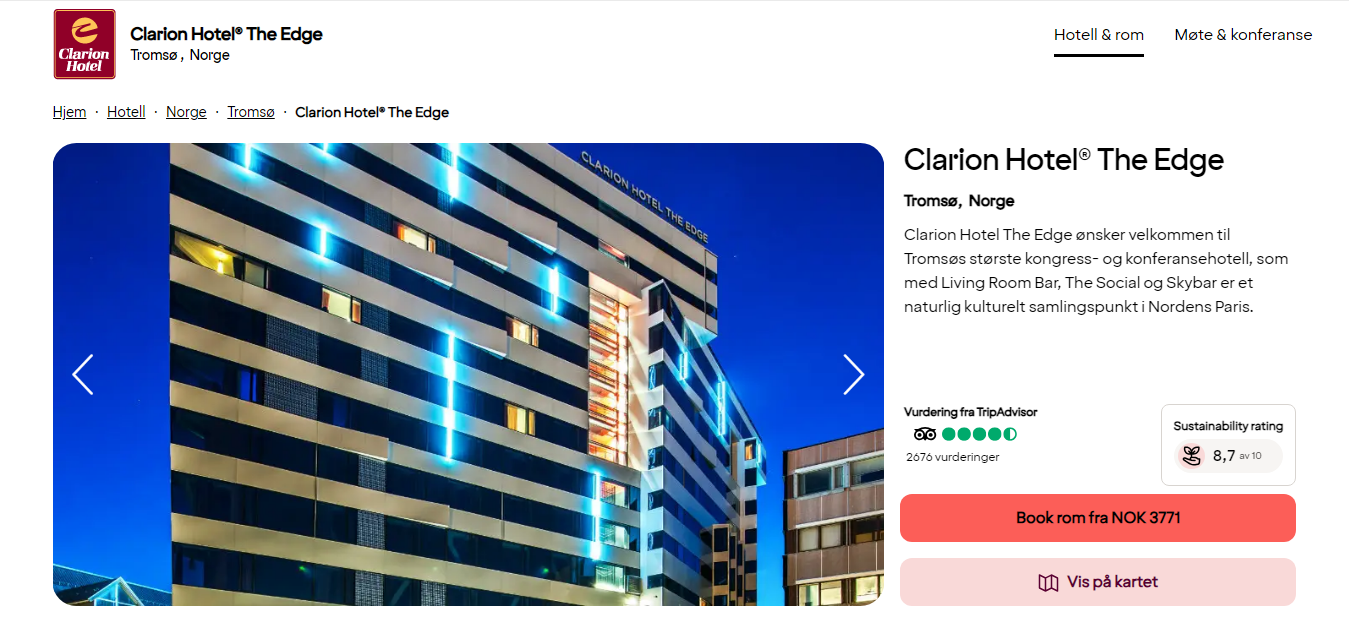
\includegraphics{dokumentobjekter/figurer/the_edge.png}

I den senere tid har Tromsø opplevd en stor økning i antall turister som
kommer til byen, og da særlig i vintersesongen. Hvor den økningen i
etterspørselen etter overnatting har resultert i en stor prisøkning på
hotellrom i vintersesongen.

I denne oppgaven skal vi svare på følgende spørsmål:

\begin{enumerate}
\def\labelenumi{\arabic{enumi}.}
\item
  Hvilken prisstrategi bruker Clarion Hotel® The Edge, og hva vil være
  optimal markedstilpasning for hotellet?
\item
  Hvordan vil prisdiskriminering basert på ulike sesonger påvirke
  lønnsomheten til Clarion Hotel® The Edge?
\item
  Hva er velferdseffekten av Clarion Hotel® The Edge sin strategi for
  prisdiskriminering? Som følge av mange direkteflyginger fra utlandet
  til Tromsø, forventes det en økning i etterspørselen etter hotellrom.
\item
  Hvordan vil en økning i etterspørselen etter hotellrom påvirke
  prisnivået for Clarion Hotel® The Edge i de ulike sesongene?
\end{enumerate}

\subsubsection{Målgrupper}\label{muxe5lgrupper}

Strawberry Hotels deler opp hotellene sine i tre forskjellige
segmenter/brands for forskjellige målgrupper. Hvor vi har Comfort for
lavpris-kjeden, Quality som familie-hotellkjeden og til sist Clarion som
deres luksuriøse hotell-kjede hvor de alle tre er rettet mot
forskjellige behov i forskjellige målgrupper (andregrads
prisdiskriminering).

Clarion Hotel® The Edge er Strawberry Hotels største hotell i Tromsø,
hvor de selv reklamerer for naturen rundt byen, diverse aktiviteter som
vi kan bestille
\href{https://www.strawberryhotels.com/packages/tromso}{samtidig med hotell-bookingen},
nordlyset osv. for å tiltrekke seg besøkende året rundt.

\newpage

\subsection{1.2 Hotellbransjen}\label{hotellbransjen}

\subsubsection{Vekst over tid}\label{vekst-over-tid}

\begin{figure}[h]
\centering
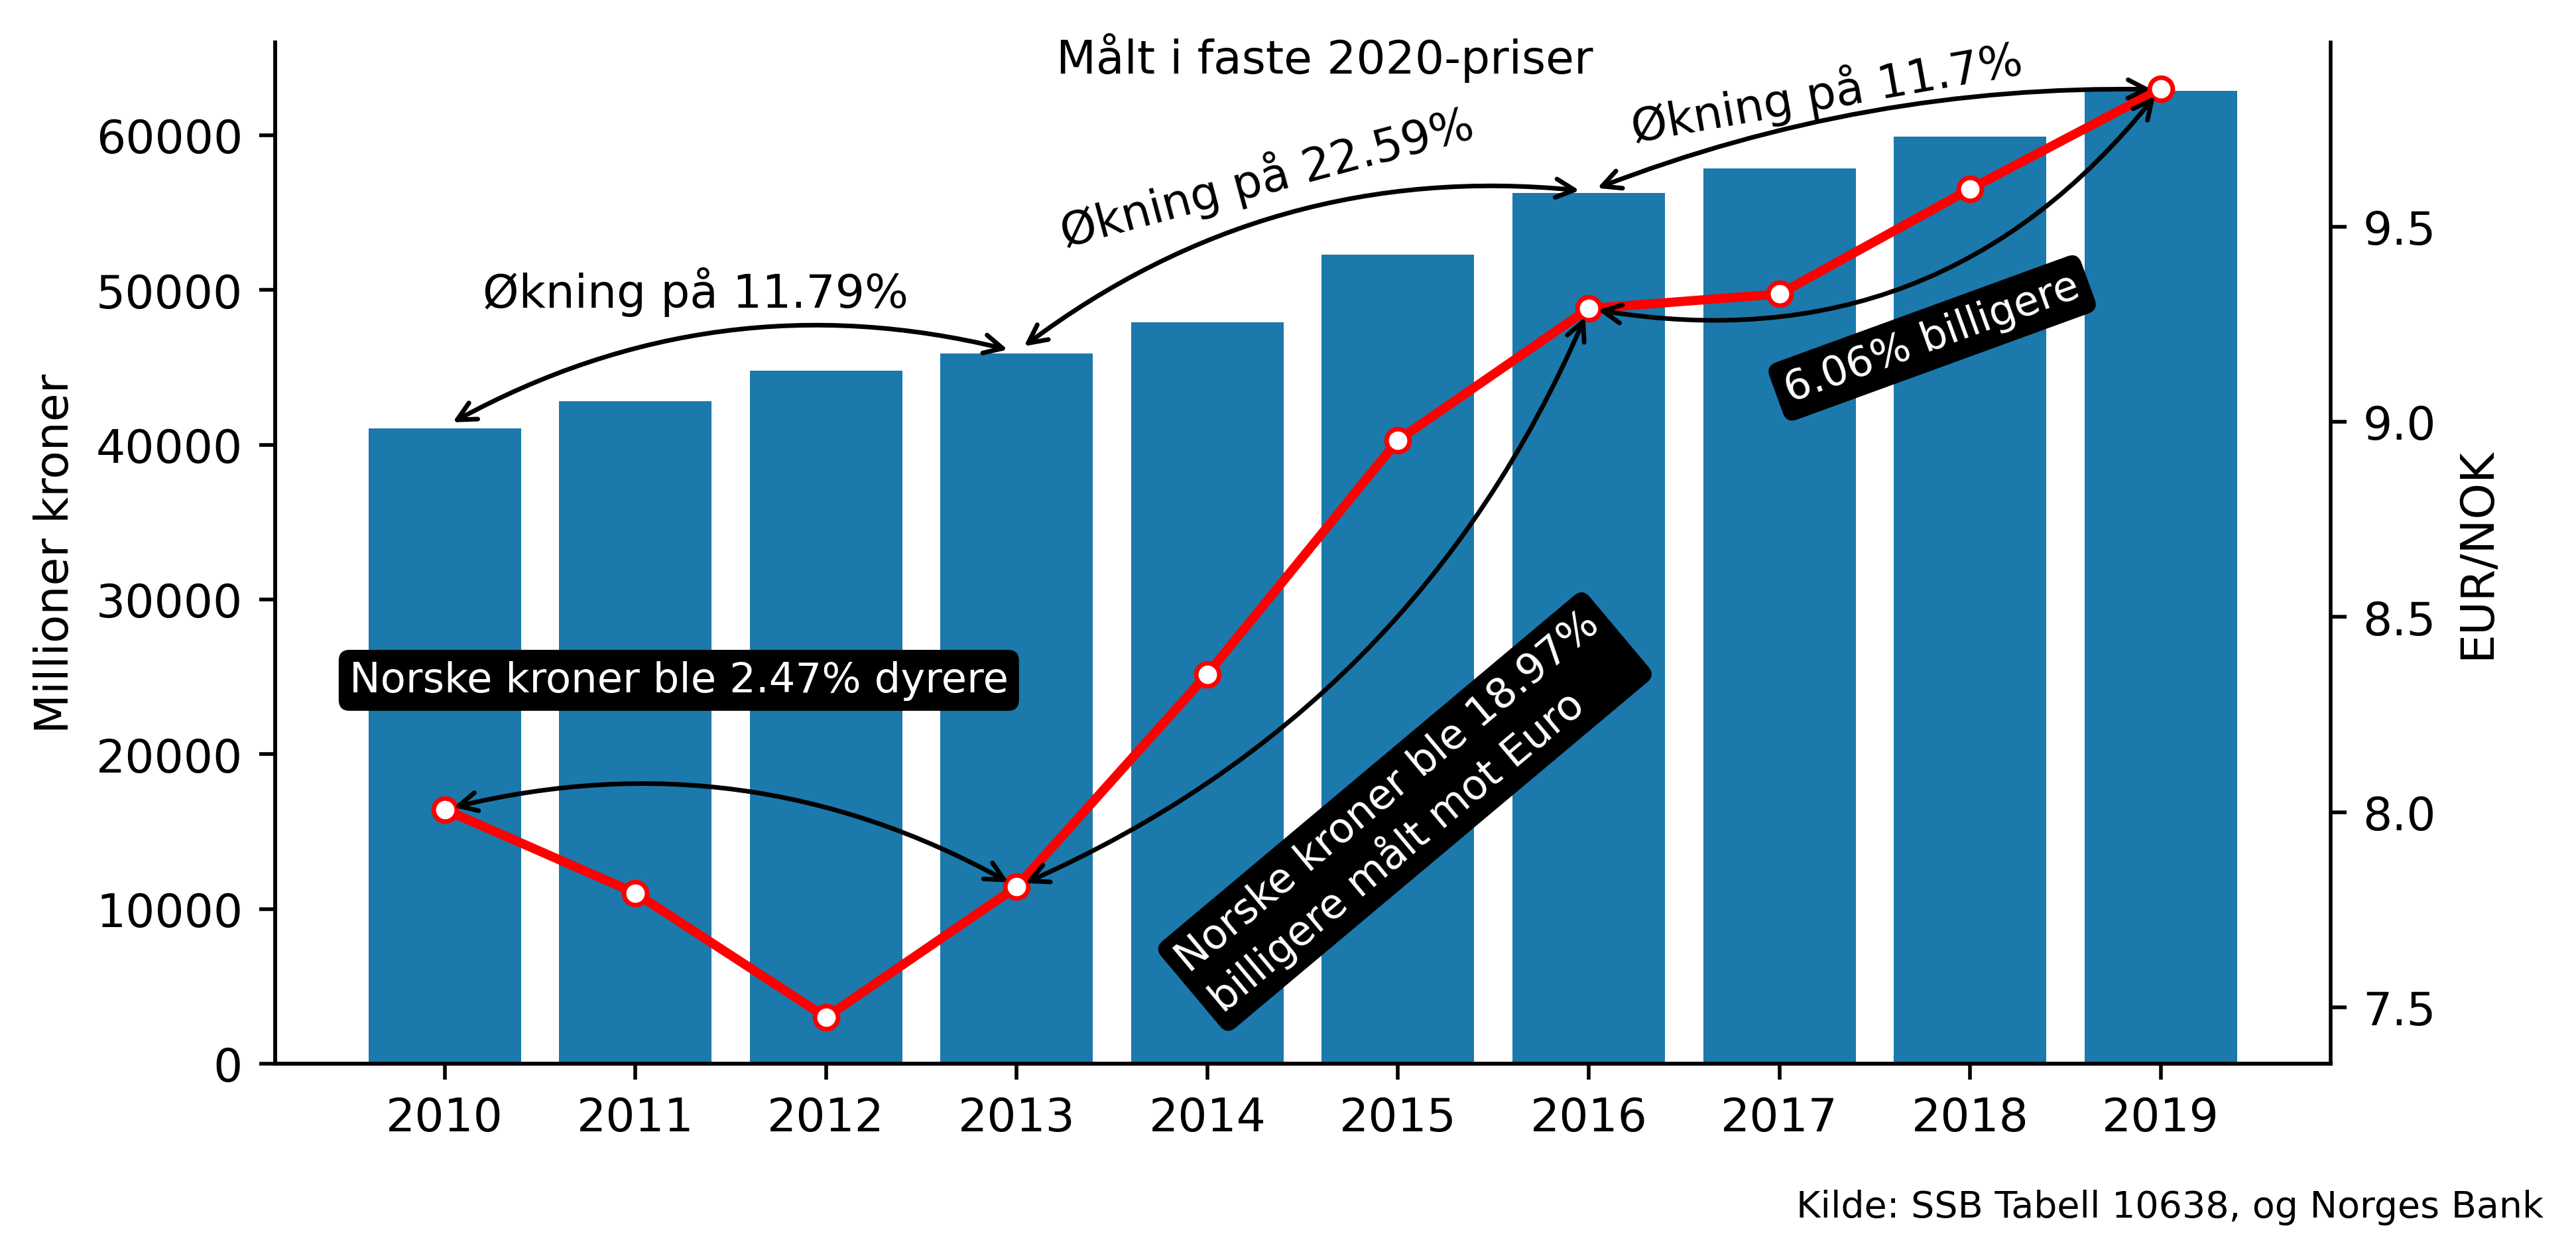
\includegraphics[width=0.8\textwidth]{dokumentobjekter/figurer/Utlendingenes_turistkonsum_i_Norge.png}
\caption{Utlendingenes turistkonsum i Norge med EUR/NOK}
\label{fig:konsum}
\end{figure}

Det siste tiåret har vi sett svekkelser i kronekursen mot utenlandske
valutaer. Svekkelsen mot både euro og dollar har gjort Norge til et mer
økonomisk attraktivt reisemål for utenlandske turister.

\begin{figure}[h]
\centering
  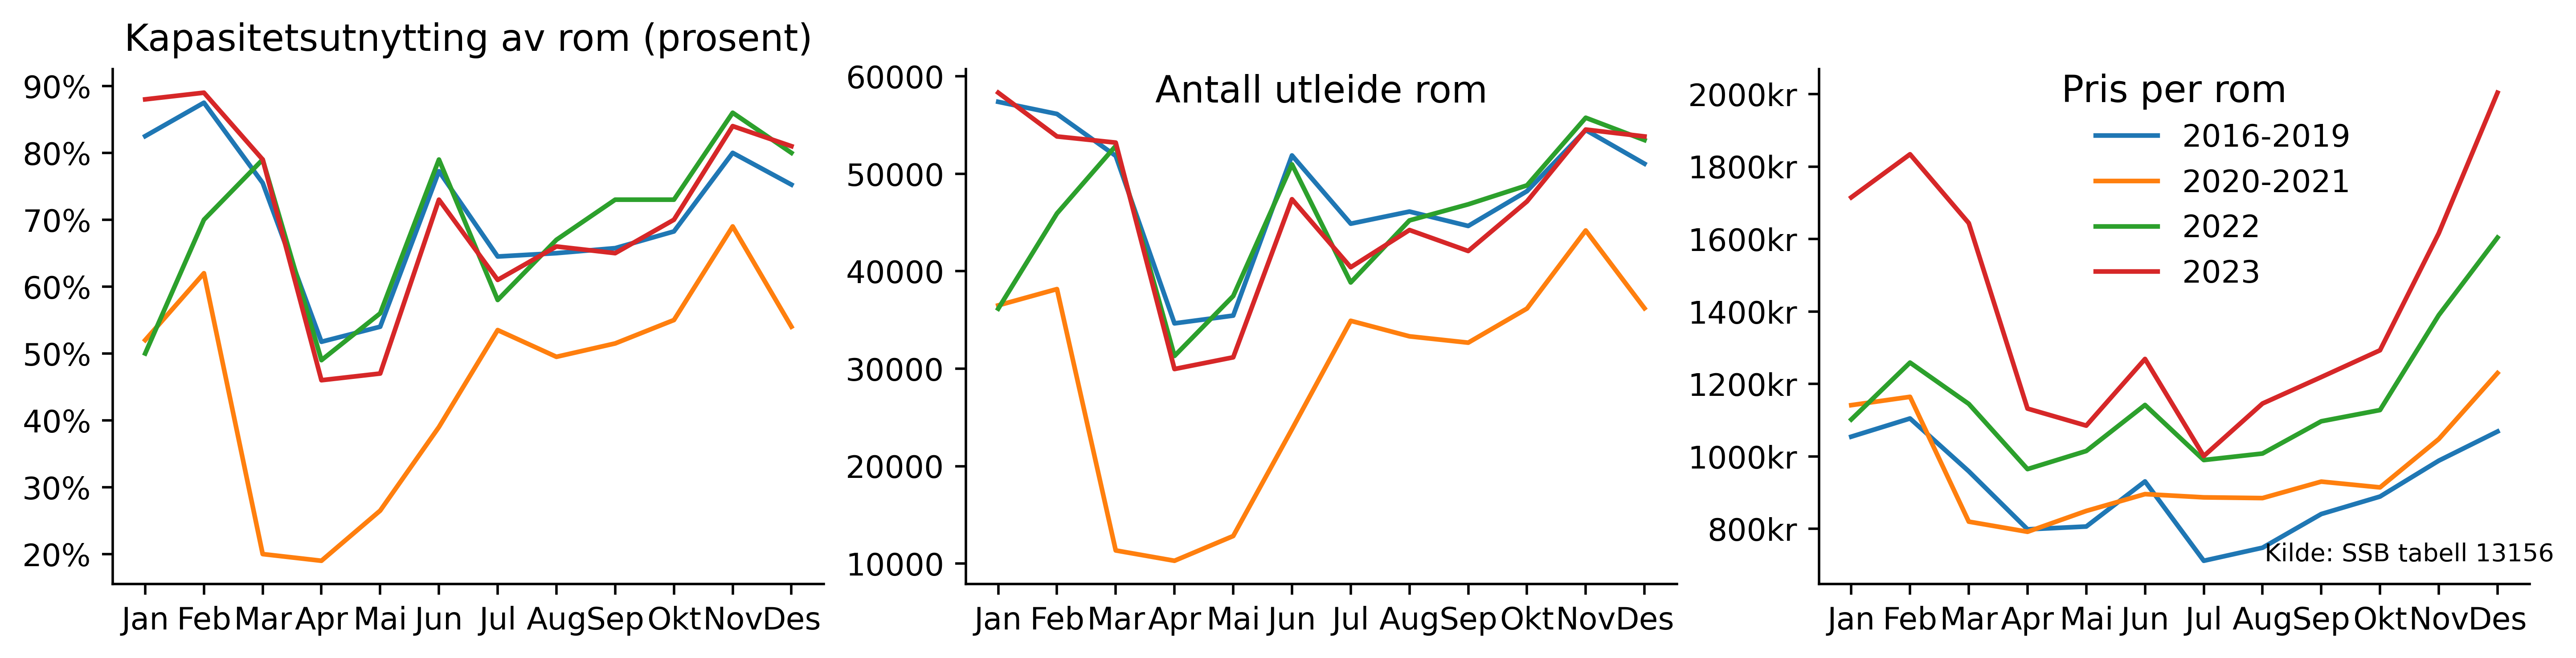
\includegraphics[width=\textwidth]{dokumentobjekter/figurer/ssbdata.png}
  \caption{Sesongvariasjoner i hotellbransjen}
  \label{fig:ssbdata}
\end{figure}

Tromsø ligger nå på topp i landet når det gjelder hotellbelegg og
oppnådd høyest pris for sine hotellrom i 2023. Totalt for året var
hotellbelegget på 68,9 prosent. For vintermånedene, fra november til
mars, ligger hotellbelegget på mellom 80 og 90 prosent.

I \autoref{fig:ssbdata} så er det tegnet 4 linjer der blå viser
gjennomsnitt av årene 2016-2019, oransje viser 2020-2021 og til slutt
viser grønn og rød 2022 og 2023. Den besluttingen ble tatt for forbedre
visualiseringen.

I sommermånedene synker etterspørselen etter overnatting betydelig, og
hotellbelegget ligger mellom 55 og 62 prosent. Clarion Hotel The Edge er
Tromsøs største kongress- og konferansehotell. Hotellet inngår i
hotellkjeden Strawberry.

Prisene i \hyperref[fig:ssbdata]{høyre figur} er justert etter
konsumprisindeksen for å forsøke å fjerne inflasjon fra prisutviklingen.
Som vi ser, selv KPI-justert så har prisene i 2023 vært en god del
høyere.\footnote{Koden fra disse figurene er i stor grad gjenbrukt kode
  fra tidligere levert mappeoppgave fra emnet SOK-1006.
  Kandidatnummer\_3 (2023)}

\clearpage

\subsection{1.3 Hva driver pris}\label{hva-driver-pris}

Som vi kan observere, er prisen på hotellrom i Tromsø relativt høy på
vinteren, og relativt lav om sommeren. Hva driver egentlig prisen? Vi
har to faktorer som driver pris i markedet: tilbud og etterspørsel.
Samspillet mellom disse skal vi se videre i teoridelen.

Prisen på hotellrom vil også kunne variere ut ifra lønn, drift,
vedlikehold, osv. Kostnaden for hotellrom er ikke bare sengetøy og vask
av rom, men driftskostnader som strøm, mat/drikke, lånekostnader, osv.

Blant annet driftsmarginer og driftskostnader kan med andre ord påvirke
prisen på hotellrom. Hotellbransjen hadde i 2022 blant de laveste
driftsmarginene av næringene i Norge. Driftsmarginen lå på 3,9 prosent i
2022, sammenlignet med generelt for alle næringer på 22 prosent.
Allikevel kan vi se en økning i marginer i forhold til før
covid-pandemien (driftsmargin i 2019 var 1,9 prosent). \footnote{\emph{Tall
  Og Fakta Om Norsk Reiseliv} (n.d.)}

Akkurat nå opplever vi en periode med økte priser grunnet inflasjon.
Dette medfører også en økt lønnsvekst, da arbeidere krever økt
kjøpekraft. Hotellbransjen har en høy andel av sine driftskostnader
knyttet til lønn. Ifølge NHO var denne på 36,9
prosent\(\color{blue}{^2}\). Dette vil si at bransjen er sensitiv til
økte lønnskostnader, og derav kan prisene justeres for å opprettholde
margin.

\paragraph{Mews PMS og The Edge.}\label{mews-pms-og-the-edge.}

Da Clarion Hotel The Edge er en del av Strawberry-gruppen, kan vi anta
at de bruker samme PMS (property managment system) som resten av
Strawberry. Dette vil si at Clarion Hotel The Edge benytter seg av
PMS-programmet Mews.\footnote{Mews (n.d.-a)}

Selv som vi ser en høyere etterspørsel under vintersesong, vil prisene
variere fra dag til dag. Mews tillater automatisk justering av priser
basert på etterspørsel. Dette vil si flere rom solgt, desto høyere vil
prisen bli. Dette baserer seg på en rate satt av hotellet i
utgangspunktet. Dette vil si at vi antar The Edge har en langt høyere
basepris under vintersesong, enn på sommeren ut ifra de observerte
prisforskjellene.\footnote{Mews (n.d.-a)}

\subsubsection{Faktorer som påvirker
etterspørsel}\label{faktorer-som-puxe5virker-etterspuxf8rsel}

Som vist i \autoref{fig:konsum}, har turistkonsumet økt, som vi kan anta
har delvis blitt drevet av denne valutaeffekten.
\hypertarget{faktorer_ettersporsel}{Hotellovernattinger
utgjør en en del av det totale turistkonsumet og prisfølsomheten i våre
etterspørselsfunksjoner som vi kommer til i kapittel 3 på -1.2 og -2.3 passer godt med observasjonene.}

I
\href{https://ntnuopen.ntnu.no/ntnu-xmlui/bitstream/handle/11250/2486498/Masteroppgave\%20Ida\%20Charlotte\%20Engebretsen.pdf}{Ida Charlotte Sølvberg Engebretsen}
sin masteroppgave fremkommer det at priselastisiteten for etterspørselen
er -0.6 på kort sikt og -2.86 på lang sikt, noe som betyr at turister er
prisfølsomme på lang sikt men ikke på kort sikt. Dette betyr at
langvarige valutatrender kan ha stor påvirkning på turiststrømmene og
den økningen vi nå har sett kan være bare starten. Med dette kan det
forventes en ytterligere økning i etterspørsel på sikt.

Fra
\href{https://www.regjeringen.no/no/dokumenter/nou-2019-11/id2645213/?ch=7}{regjeringens NOU}
ser vi at etterspørselselastisiteten i totalmarkedet for hotell benyttes
på -0,9, nær korttidsestimeringen i Engebretsens oppgave og
sommerelastisiteten vi har. Dette støtter vår antagelse om at
kronesvekkelsen vil føre til en økt etterspørsel etter hotelltjenester.

Vi har ikke funnet noe for å støtte det men vi fikk høre av daglig leder
på The Edge at utenlandske turister har høyere betalingsvillighet enn
nordmenn. Dette kan bety at utenlandske turister kan være villig til å
betale mer for et hotellrom enn nordmenn. Dette kan være en faktor som
påvirker prisen på hotellrom i Tromsø.

De siste årene har temperaturen i Europa økt, med flere hetebølger som
kan føre til at flere turister vil reise nordover for å unnslippe varmen
på sommeren slik at det kan bli mer balansert etterspørsel på sommer og
vinter.

\paragraph{Oppsumert}\label{oppsumert}

I denne oppgaven vil vi se på effekten av tredje grads
prisdiskriminering, hvor Clarion Hotel® The Edge prøver å differensiere
prisen mellom vinter- og sommersesongen.

Vi ser bare på etterspørselssiden og ser i stor grad bort ifra
tilbudssiden selv om det på sikt kan bygges nye hoteller. Vi velger også
å bare se på hoteller og ikke på AirBnB. Vi betrakter også The Edge som
en monopolist i markedet da de er en av de eneste luksushotellene i
Tromsø.

Vi gå også ut ifra at det er lineær etterspørsel der vi setter en fast
for sommer og vinter. Men som vi ser er det veldig mange faktorer som
påvirker pris, og med så mange pakker hoteller kan tilby, foreksempel
som samarbeid med flyselskap som Norwegian og forskjellige hotell for
forskjellige markedssegmenter. Derfor gjør vi en avgrensing der vi bare
ser på tredjegrads prisdiskriminering

\subsection{1.4 Struktur av oppgaven}\label{struktur-av-oppgaven}

\paragraph{Kapittel 1}\label{kapittel-1}

I kapittel 1 har vi presentert bakgrunnen for oppgaven, og vi har også
presentert problemstillingen som vi skal forsøke å besvare i denne
oppgaven. Vi har også vist data på turisme og hotellbransjen og fortalt
om avgrensningene vi har gjort, og vi presenterer her strukturen av
oppgaven.

\paragraph{Kapittel 2}\label{kapittel-2}

I kapittel 2 går vi gjennom den teoretiske delen av oppgaven, hvor vi
forklarer monopol, frikonkurranse, velferdseffekter av disse og
presenterer teorien bak prisdiskriminering. Vi fokuserer spesielt på
tredje grads prisdiskriminering, som er den prisdiskrimineringen vi skal
se på i denne oppgaven.

\paragraph{Kapittel 3}\label{kapittel-3}

Kapittel 3 inneholder analysen hvor vi ser på hvilken effekt det vil ha
å ikke prisdiskriminere, og hvilken effekt det vil ha å
prisdiskriminere. Vi vil også se på hvordan The Edge kan differensiere
prisen mellom vinter- og sommersesongen. Vi vil også se på hvilke
velferdseffekter dette vil ha for samfunnet. Vi avslutter der vi drøfter
rundt hvilke effekter vi ser og hva vi kan forvente.

\paragraph{Kapittel 4}\label{kapittel-4}

I kapittel 4 konkluderer vi med at den optimale prisstrategien en er en
differensiert prissetting basert på sesong.

\clearpage

\section{2. Teorikapittel}\label{teorikapittel}

Før vi begynner å se på prisstrategien til hotellet Clarion Hotel® The
Edge, skal vi gå gjennom hvordan en bedrift som har monopolmakt
profittmaksimerer, hvordan ulike former for prisdiskriminering fungerer
og hvilke velferds-effekter monopol har for samfunnet i helhet.

\subsection{2.1 Frikonkurranse og
monopol}\label{frikonkurranse-og-monopol}

I vår analyse skal vi gå gjennom to markedssituasjoner: frikonkurranse
og monopol. Da vi antar The Edge har en monopol markedssituasjon, vil vi
i stor grad vektlegge dette. Vi skal alikevell gå igjennom
frikonkurranse for å se hvilke velferdseffekter en monopol
markedssituasjon har.

\subsubsection{Frikonkurranse}\label{frikonkurranse}

Det gjøres noen forutsetninger for å kunne ta hensyn til frikonkurranse.
Disse er at alle bedriftene produserer samme produkt/tjeneste,
fullkommen informasjon (lik informasjon hos tilbydere/konsumenter),
mange aktører på markedet og ingen transaksjonskostnader. Da disse
forutsetningene er satt, skal vi se på hvordan markedskreftene fungerer.

Ved frikonkurranse har vi to faktorer som driver markedspris for et
gode: tilbud og etterspørsel. Tilbudet representerer marginalkostnaden
til bedriftene for å produsere godet. Dette vil si at tilbudet
gjenspeiler kostnaden ved produksjon av varen/varene. Etterspørselen
representerer betalingsvilligheten til konsumentene (altså hvor mye
individene er villig til å betale). Desto lavere pris, desto flere
ønsker å kjøpe godet, noe som etterspørselkurven viser. Figuren nedenfor
viser hvordan tilbud og etterspørsel møtes, gjerne kalt markedslikevekt.

\begin{figure}[h!]
\centering
  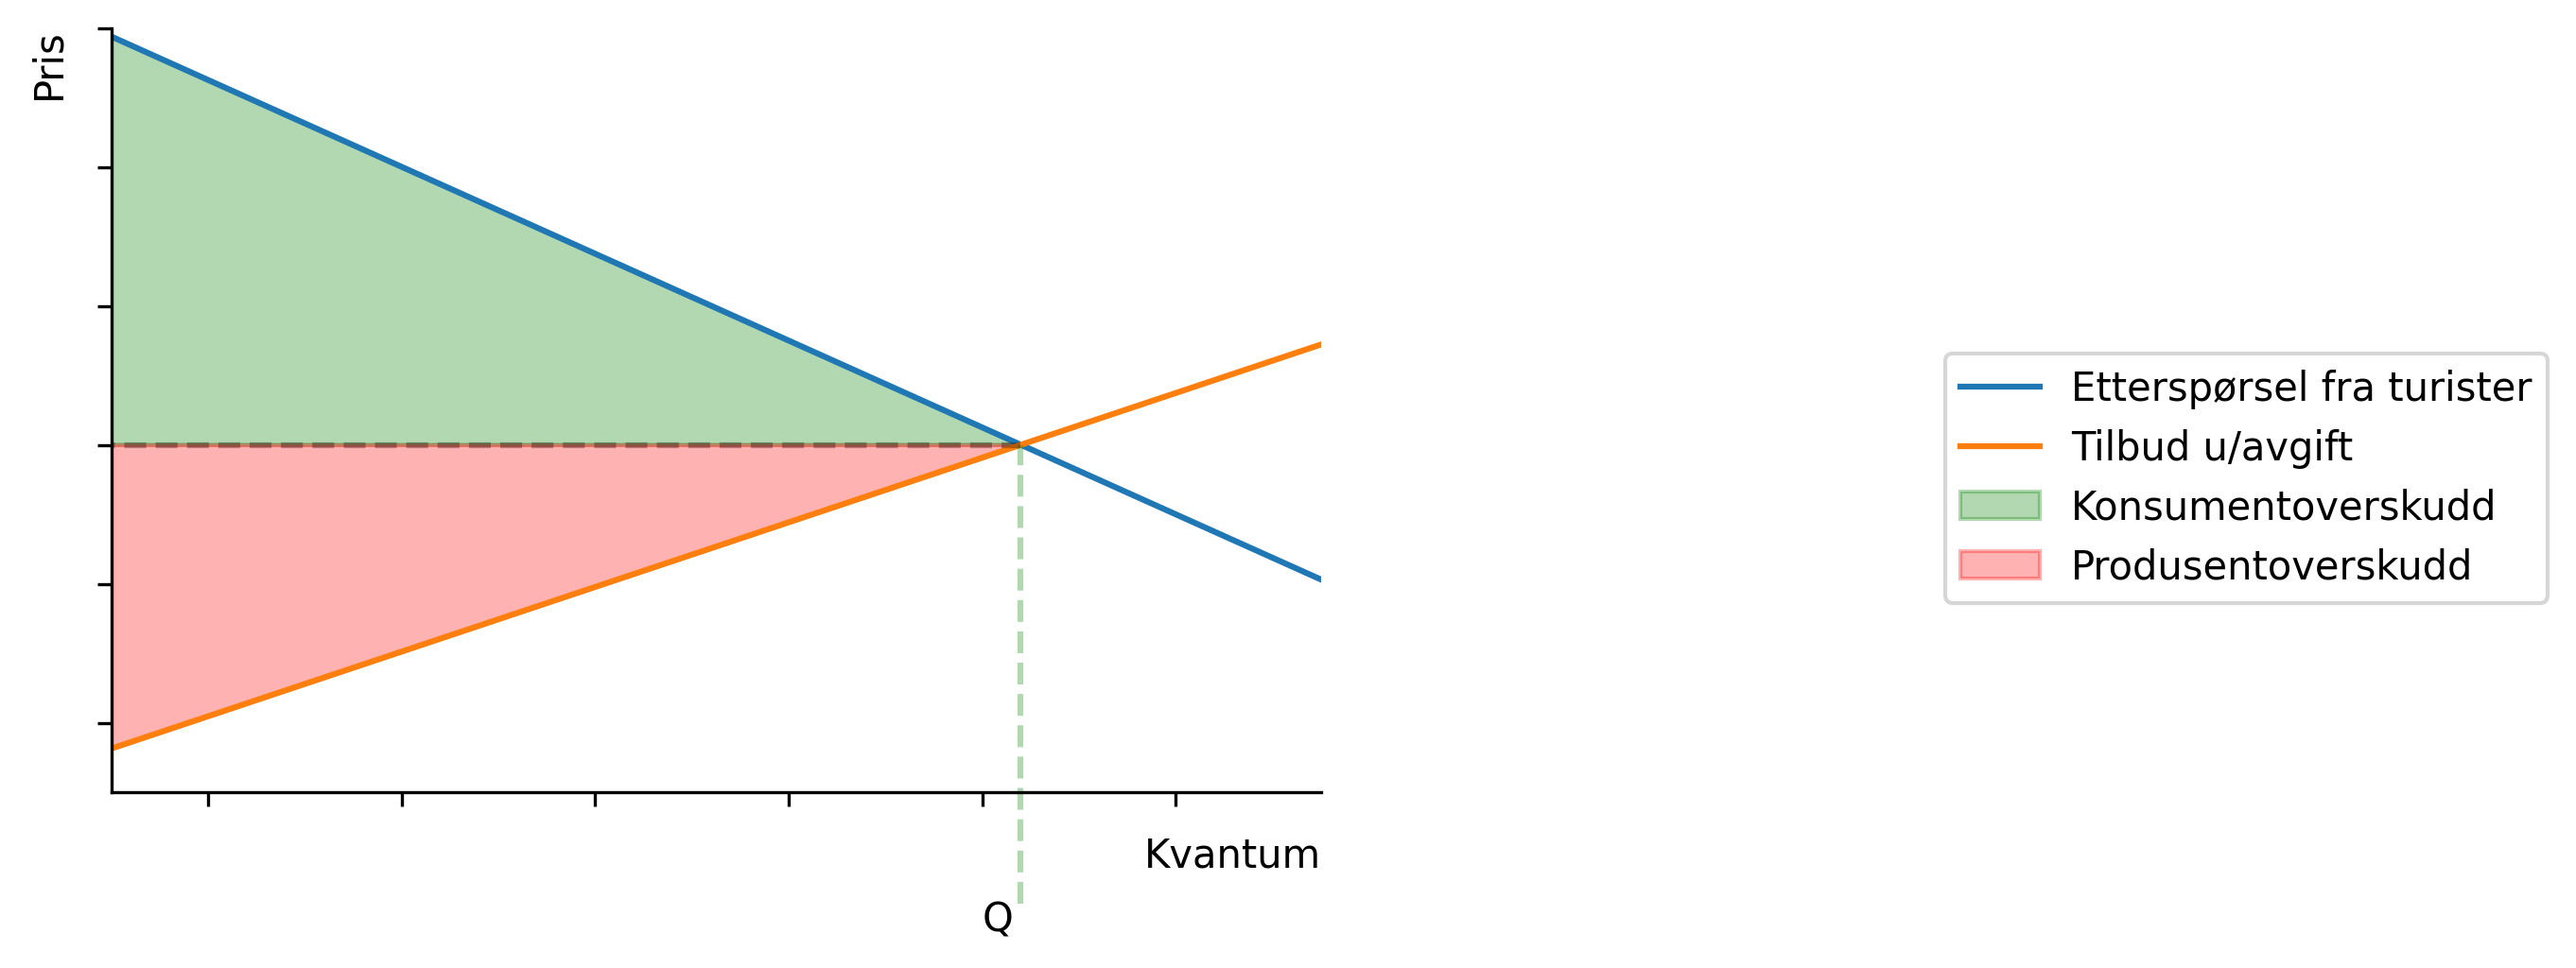
\includegraphics[width=\linewidth]{dokumentobjekter/figurer/frikonkurranse.png}
  \captionof{figure}{Frikonkurranse}
  \label{fig:frikonkurranse}
\end{figure}

\autoref{fig:frikonkurranse} viser hvordan samspillet mellom tilbud og
etterspørsel. Punktet hvor disse tangerer kalles markedslikevekt, og er
samfunnsøkonomisk optimalt. Samfunnsøkonomisk optimal tilpasning er når
samfunnsøkonomisk overskudd er maksimert, og består av produsent- og
konsumentoverskudd. Konsumentoverskudd får vi når konsumentene betaler
mindre enn hva de har betalingsvillighet til (dette illustreres med det
grønne området i figuren). Produsentoverskuddet er det røde området i
figuren, og representerer overskuddet bedriften/produsenten får ved å
produsere frem til likevektspris (altså merinntekt utover
marginalkostnaden ved å produsere godet). Produsent- og
konsumentoverskuddet utgjør det samfunnsøkonomiske overskuddet, og dette
er maksimert når tilbud og etterspørsel tangerer.

\subsubsection{Monopol}\label{monopol}

Et monopol vil si at vi har en markedsituasjon hvor det finnes bare en
bedrift på tilbudssiden. I motsetning til fullkommen konkurranse hvor
prisen blir satt av markedet og bedriften er pristagere, kan en bedrift
med monopolmakt bestemme prisen selv. Da monopol-bedriften ønsker å
profittmaksimere, vil denne selvsagt velge prisen som maksimerer profitt
uten å se på samfunnsøkonomisk velferd.

\subsection{2.2 Profittmaksimering i en bedrift som har
monopol}\label{profittmaksimering-i-en-bedrift-som-har-monopol}

En bedrift med monopolmakt vil velge en tilpasning som maksimerer dens
profitt utifra en gitt etterspørsel etter deres produkt/tjeneste. La oss
starte med en generell invers etterspørselsfunksjon, da
monopol-bedriften kan velge prisen selv: \[ P(Q) = A - BQ\]Den inverse
etterspørselsfunksjonen viser sammenhengen mellom pris (\(P\)) og mengde
solgt (\(Q\)). Konstantleddet \(A\) representerer prisen som medfører
null etterspørsel etter produktet/tjenesten bedriften selger. \(B\)
representerer hvor mye prisen endrer seg dersom etterspørselen endres
med \(1\) enhet.

Da bedriften har monopol, vil denne være eneste tilbyder til markedet.
Dette vil si at bedriften vil dekke hele markedet. Dette gir bedriften
en inntekts-funksjon som ser slik ut: \[R(Q) = Q * P(Q)\]Inntekten
\(R(Q)\) avhenger av antall solgt (\(Q\)) til en pris \(P\). Da
bedriften dekker hele markedet vil prisen være den inverse
etterspørselen \(P(Q)\). Videre forenkler vi likningen og får følgende
inntekts-funksjon for monopolbedriften:

\[R(Q) = Q * P(Q) \rightarrow R(Q) = Q * (A-BQ) \rightarrow R(Q) = AQ -BQ^2\]

Bedriften har også en kostnadsfunksjon, som representerer kostnaden for
enheter produsert. Denne kan se slik ut: \(C(Q) = c * Q\), hvor \(c\) er
enhetskostnaden for hver enhet produsert/levert. Dette vil si at det
koster \(c\) kroner å produsere en ekstra enhet av produktet/tjenesten.
I tillegg har gjerne bedriften faste kostnader \(F\).

Monopol-bedriftens profittfunksjon \(\pi(Q)\) vil dermed se slik ut:

\[\pi(Q) = R(Q) - C(Q) - F \rightarrow \pi(Q) = AQ - BQ^2 - cQ - F\]

Monopolbedriften vil selge flere produkter/tjenester så lenge de tjener
penger på dette. Dette vil si at bedriften vil selge enheter frem til
\(\frac{\delta\pi(Q)}{\delta Q} = 0\) for å oppnå maksimal profitt.

\[\frac{\delta\pi(Q)}{\delta Q} = 0 \rightarrow A-2BQ - c = 0 \rightarrow A - 2BQ = c \rightarrow MR = MC\]MR
står for marginalrevenue, eller marginalinntekt på norsk. Dette er
inntekten bedriften får ved å selge en ekstra enhet (altså
\(MR = \frac{\delta R(Q)}{\delta Q} \rightarrow MR = A-2BQ\)). Her kan
vi se at marginalinntekten er lik den originale etterspørselfunksjonen
vår \(P(Q)\), utenom helningen som er dobbelt så bratt som
etterspørselens. Dette prinsippet kommer til å bli brukt for å forenkle
under analysedelen. MC står for marginalcost, eller marginalkostnad på
norsk. Dette er kostnaden for bedriften ved å produsere en ekstra enhet
(\(MC = \frac{\delta C(Q)}{\delta Q} \rightarrow MC = c\)). Hva
forteller dette oss om monopolbedriftens vilkår for profittmaksimering?

Monopolbedriften profittmaksimerer altså når marginalinntekten \(MR\) er
lik marginalkostnaden \(MC\). Dette forteller oss at monopol-bedriften
profittmaksimerer når følgende vilkår er oppfylt:
\(MR = MC \rightarrow A-2BQ = c\). Legg gjerne merke til at \(A\) og
\(B\) kommer fra den opprinnelige etterspørselsfunksjonen.

\begin{figure}[h!]
\centering
  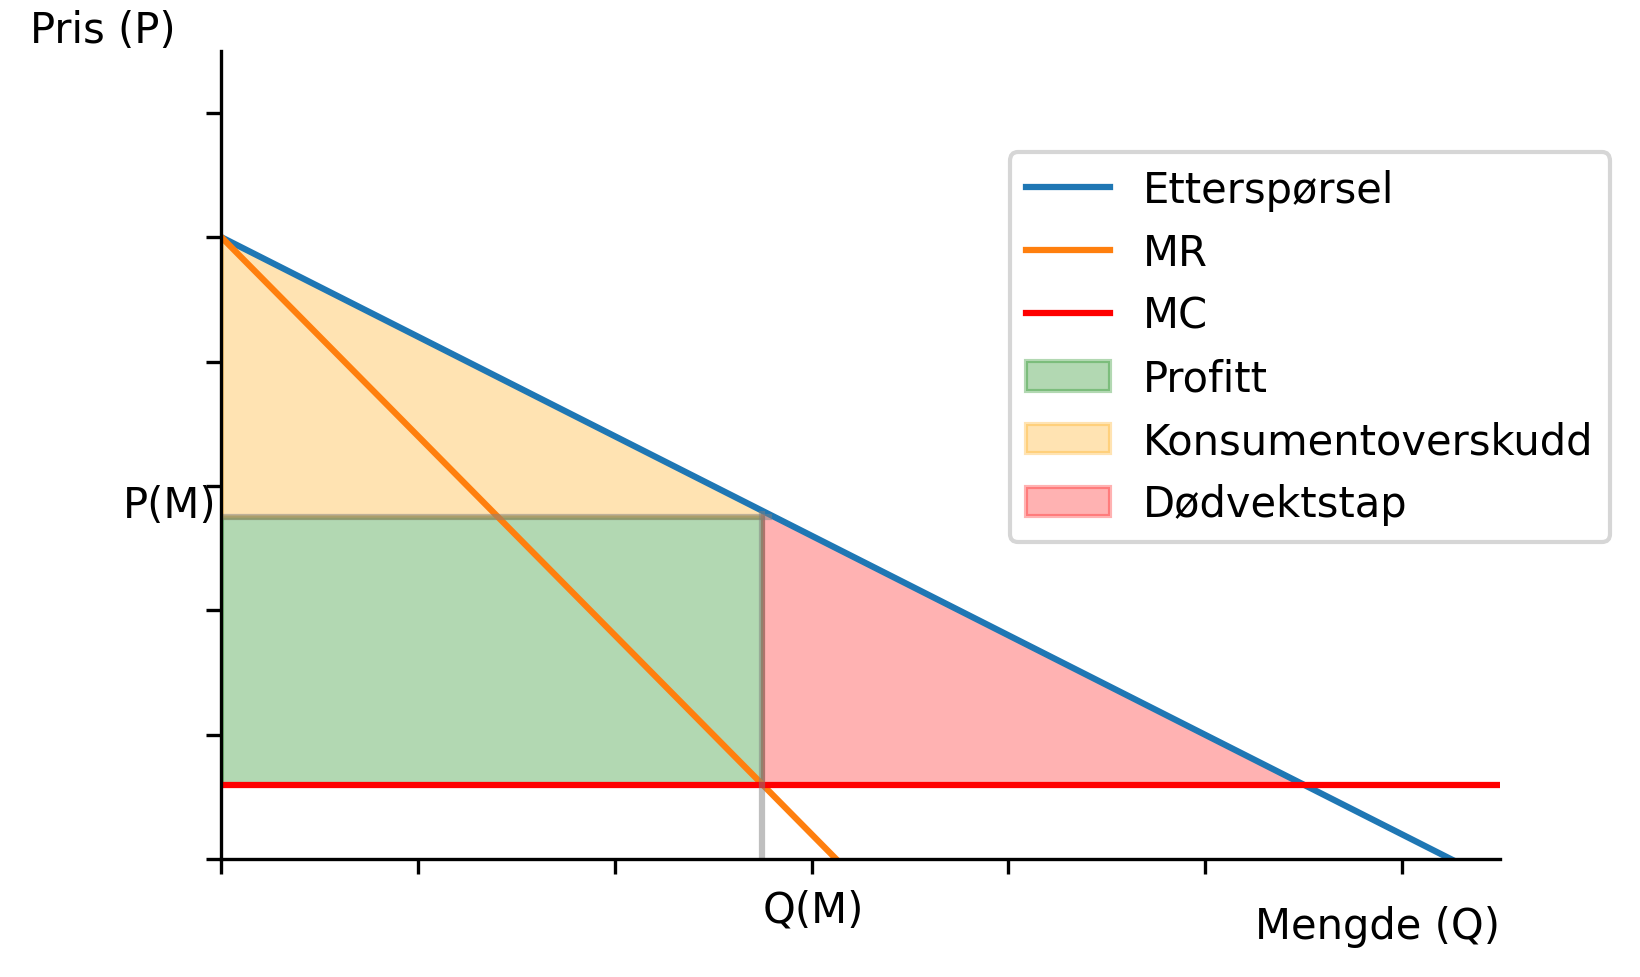
\includegraphics[width=\linewidth]{dokumentobjekter/figurer/monopol.png}
  \captionof{figure}{Monopol tilpasning}
  \label{fig:monopol}
\end{figure}

\autoref{fig:monopol} viser hvordan bedriften med monopolmakt vil
tilpasse seg. I eksempelfiguren har en antatt at marginalkostnaden er
konstant \(c\).

I \autoref{fig:monopol} kan vi se at monopolbedriften vil selge \(Q(M)\)
mengde enheter til en pris \(P(M)\), da dette oppfyller vilkåret for
profittmaksimering hvorav \(MR = MC\) (en kan se i figuren hvor \(MR\)
og \(MC\) tangerer hverandre). Det grønne området vil representere
monopol-bedriftens profitt \(\pi\). Ved fullkommen konkurranse der
prisen er gitt av markedet, ville tilpasset seg ved å selge frem til
prisen er lik marginalkostnaden, altså \(P = MC\). Grunnet at bedriften
er eneste tilbyder av godet, vil en velge å profittmaksimere, og derav
selge et lavere kvantum enn hva som er samfunnsøkonomisk optimalt. Dette
medfører ett dødvektstap, som en kan se i figuren markert med rødt
område (ett effektivitetstap grunnet lavere kvantum enn samfunnet
etterspør til \(P=MC\)).En kan også se et konsumentoverskudd som er
markert gult. Dette vil si at noen konsumenter får kjøpe godet til
lavere pris enn hva de har betalingsvillighet for, som gir oss dette
konsumentoverskuddet.

\subsubsection{Monopoltilpasning dersom kundene har ulik
betalingsvillighet}\label{monopoltilpasning-dersom-kundene-har-ulik-betalingsvillighet}

Monopolisten kan stå ovenfor kundegrupper med ulik betalingsvillighet.
La oss se hvordan monopol-bedriften tilpasser seg dette:

\begin{figure}[h!]
\centering
  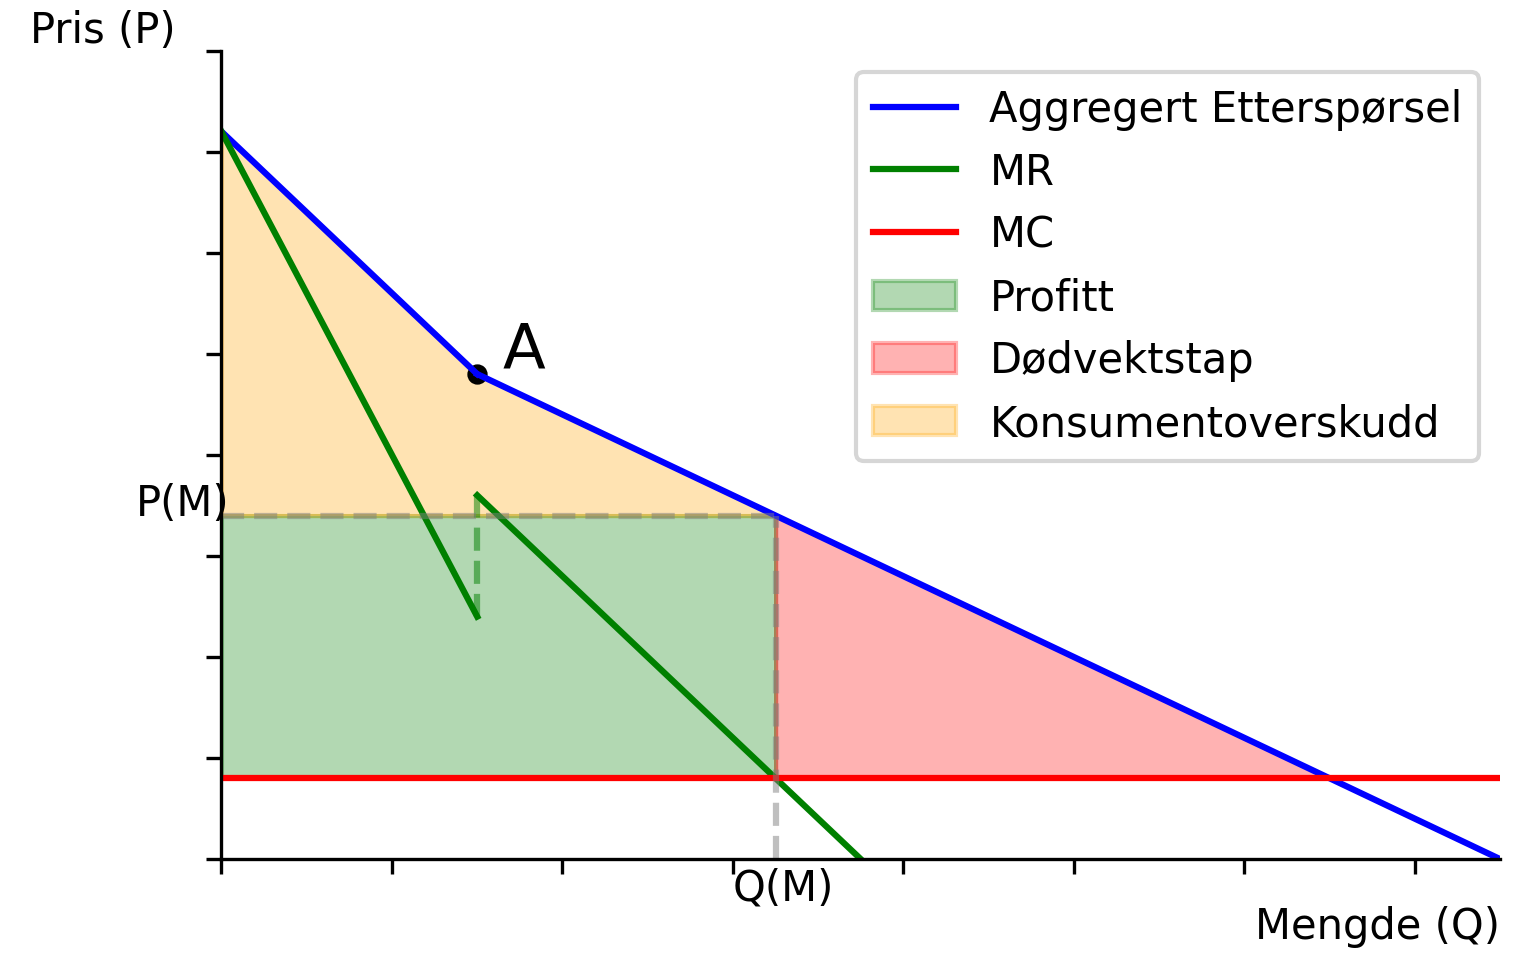
\includegraphics[width=\linewidth]{dokumentobjekter/figurer/bedrift_tilplasning.png}
  \captionof{figure}{Bedriften tilpasser seg ved aggregert etterspørsel}
  \label{fig:tilpasning}
\end{figure}

\autoref{fig:tilpasning} viser hvordan monopol-bedriften tilpasser seg
ved aggregert etterspørsel. En aggregert etterspørsel vil si den totale
etterspørselen. I figuren kan vi se en knekk i etterspørsel vist ved
punkt A, grunnet ulik betalingsvillighet blant konsumentene. Før knekken
er etterspørselen fra gruppen/karakteristika hvor det er høy
betalingsvillighet. Etter knekken ser vi den adderte etterspørselen
mellom de med høy og lav betalingsvillighet. Optimal tilpasning vil
fortsatt være hvor marginalinntekten er lik marginalkostnaden som
figuren viser.

\subsection{2.3 Frikonkurranse vs Monopol -
Velferdseffekter}\label{frikonkurranse-vs-monopol---velferdseffekter}

Som vi kunne se ved frikonkurranse var det bedriftenes marginalkostnader
som utgjorde tilbudet. Etterspørselen utgjorde det totale etterspurte
kvantum.

Ved en monopol markedssituasjon, har vi bare en tilbyder av godet.
Monopol-bedriften vil som vi kunne se tidligere i teoridelen, tilpasse
seg ved å profittmaksimere. Dette medfører at bedriften selger enheter
frem til marginalinntekten er lik marginalkostnaden. Sammenligner vi
dette mot fullkommen konkurranse så selger bedriftene enheter frem til
prisen utgjør marginalkostnaden.

Dette medfører at monopolisten vil redusere kvantum med hensyn på å
profittmaksimere. Kvantumet reduseres, og prisen blir høyere (da
monopolisten har prisingsmakt). Dette vil ikke være samfunnsøkonomisk
optimalt, da samfunnet ikke får kjøpt enheter som ville blitt solgt om
situasjonen var fullkommen konkurranse. Dette vil si at vi får et
dødsvektstap eller effektivitetstap, grunnet det reduserte kvantumet
markedet ikke får tilgang til grunnet monopolsituasjonen.

\clearpage

\subsection{2.4 Prisdiskriminering ved
monopol}\label{prisdiskriminering-ved-monopol}

Når vi har en markedssituasjon med monopol, kan monopol-bedriften prøve
å hente ut ytterligere overskudd (og dermed øke sin profitt) hos
konsumenten ved å benytte ulike former for prisdiskriminering. Det
finnes tre ulike grader av prisdiskriminering. Første grads
prisdiskriminering (også kalt perfekt prisdiskriminering) vil si at
bedriften kjenner betalingsvilligheten til hver enkel kunde. Dette betyr
at konsumenten betaler sin marginale betalingsvillighet (det en er
villig å betale for tjenesten/produktet monopol-bedriften tilbyr). Det
finnes også prisdiskriminering av andre grad, hvor monopol-bedriften vet
at kundene har ulik betalingsvillighet. Her vil bedriften prøve å tilby
ulike pakkeløsninger/produktpakker for å la kundene selv velge hva de er
villige å betale for.

Siste form for prisdiskriminering er tredjegrads prisdiskriminering,
hvor monopol-bedriften vil skille mellom ulike segmenter gjennom
observerbare karakteristika. Dette vil si at bedriften tilbyr ulik pris
basert på et observerbart karaktertrekk. Dette kan eksempelvis være
kundens alder, student/ikke-student, militærrabatter, sesongpriser, osv.
Her ser vi hvordan monopol-bedriften skiller på disse ulike
karakteristika, ved å benytte tredjegrads prisdiskriminering:

\begin{figure}
\centering
\begin{subfigure}{.5\textwidth}
  \centering
  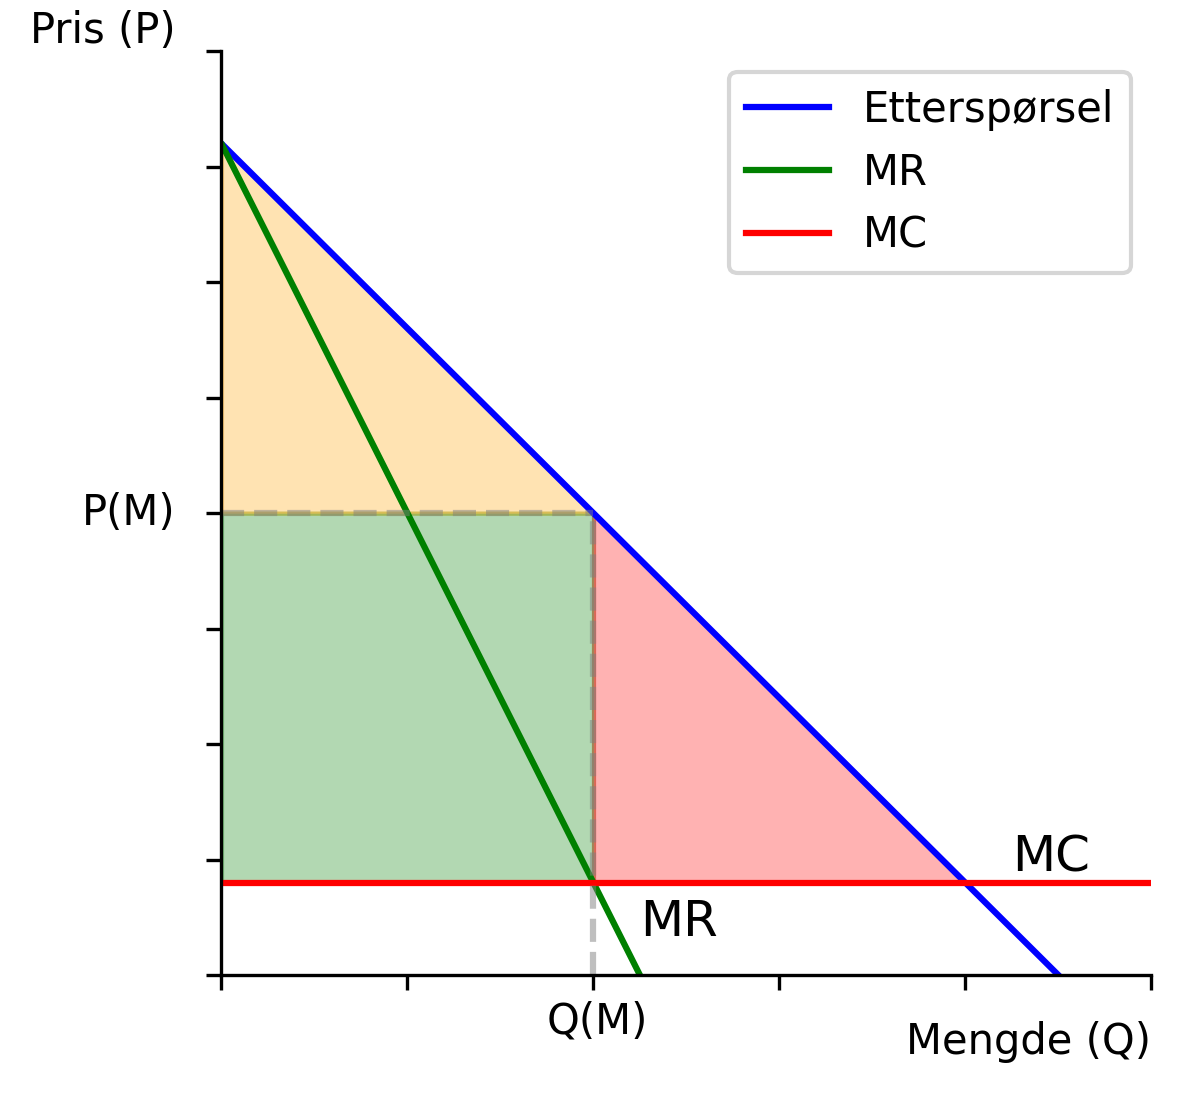
\includegraphics[width=.9\linewidth]{dokumentobjekter/figurer/hoy_betaling.png}
  \caption{Høy betalingsvillighet}
  \label{fig:hoy_betaling}
\end{subfigure}%
\begin{subfigure}{.5\textwidth}
  \centering
  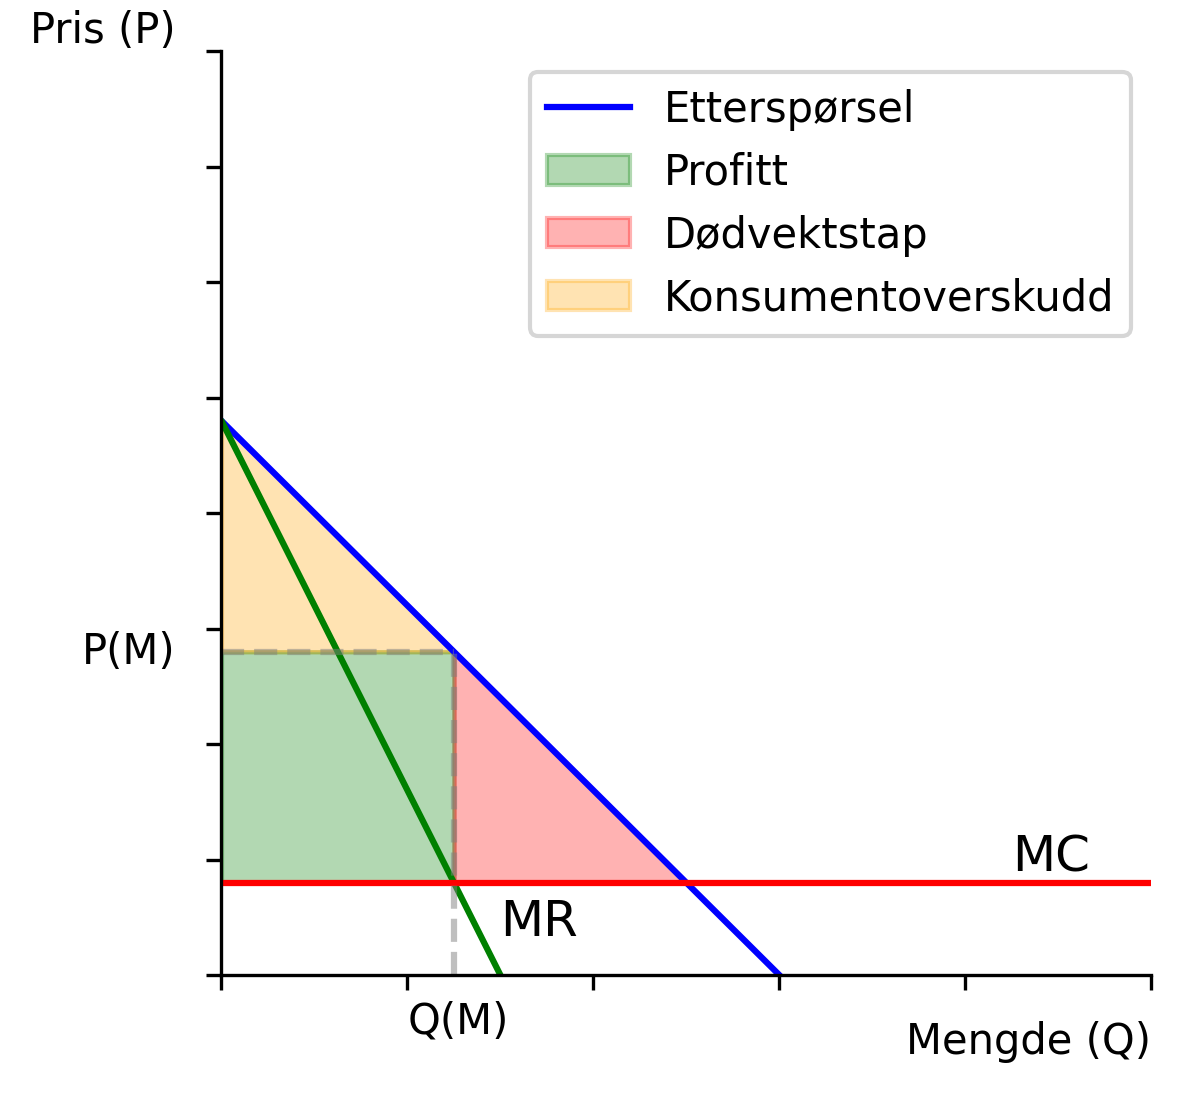
\includegraphics[width=.9\linewidth]{dokumentobjekter/figurer/lav_betaling.png}
  \caption{Lav betalingsvillighet}
  \label{fig:lav_betaling}
\end{subfigure}
\caption{Prisdiskriminering ved monopol}
\label{fig:prisdiskrimineringsfigurer}
\end{figure}

Her skiller bedriften gruppene utifra deres betalingsvillighet.
Bedriften tar en høyere pris hos gruppen med høy betalingsvillighet i
\autoref{fig:hoy_betaling} og en lavere pris hos gruppen ved lavere
betalingsvillighet vist i \autoref{fig:lav_betaling}. Bedriften ønsker å
skille betalingsvillighet (som etterspørselen gjenspeiler) for å kunne
maksimere egen profitt. Ved å skille på observerbart karakteristika kan
bedriften øke sin profitt ved å tilby en høyere pris til gruppen med høy
betalingsvillighet og en lavere til de med lav betalingsvillighet.

\clearpage

\subsection{2.5 Effekten av pris på
etterspørsel}\label{effekten-av-pris-puxe5-etterspuxf8rsel}

\subsubsection{Elastisitetsbegrepet}\label{elastisitetsbegrepet}

Elastisitet er et begrep som beskriver hvor hvor mye en variabel som
tilbud eller etterspørsel, reagerer på endringer i en annen variabel som
pris. Priselastisitet er et mål som viser hvor følsomme kjøpere og
selgere er ovenfor endringer i pris. Det viser prosentvis endring i
etterspørsel som følge av en prosentvis endring i pris. For eksempel,
hvis vi ser på priselastisiteten for et produkt og finner at den er
-0.5, betyr dette at hvis prisen øker med 1\%, vil etterspørselen falle
med 0.5\%. Priselastisitet kan være negativ, positiv eller nøytral. Hvis
priselastisiteten er negativ, vil etterspørselen falle når prisen øker.
Hvis priselastisiteten er positiv, vil etterspørselen øke når prisen
øker. Hvis priselastisiteten er nøytral, vil etterspørselen forbli
uendret når prisen endres.

Hvis 1\% økning i pris fører til mindre enn 1\% fall i etterspørsel vil
vi si at etterspørselen er inelastisk. Hvis 1\% økning i pris fører til
mer enn 1\% fall i etterspørsel vil vi si at etterspørselen er elastisk.
Hvis 1\% økning i pris fører til 1\% fall i etterspørsel vil vi si at
etterspørselen er nøytral. Men vi vil normalt ikke se på nøytral
etterspørsel da det ikke gir oss noe informasjon.

I figurer så vil helningen på etterspørselen fortelle deg noe om
etterspørselselastisiteten. Hvis etterspørselen er bratt vil det si at
etterspørselen er inelastisk og en prisendring vil ikke ha stor effekt
på kvantum mens hvis etterspørselen er flat vil det si at etterspørselen
er elastisk og det vil ha en stor effekt på kvantum solgt..

Vi kommer til å se på etterspørselssiden så vi fokuserer på
etterspørselselastisiteten og går ikke inn på tilbudssiden.

\subsubsection{Endringer i
etterspørsel}\label{endringer-i-etterspuxf8rsel}

Endringer i etterspørselen i for utenlandsk turisme til Norge kan være
påvirket av endringer i inntekt, preferanser, prisene på alternativ
turist-destinasjoner og forventninger til fremtidige prisendringer.
Dette kan føre til en forskyvning av etterspørselskurven for for
eksempel hotellrom, enten gjennom en parallel forskyvning eller med å
endre kurvens helning som ville vært en endring i etterspørselens
elastisitet.

En parallell forskyvning av etterspørselskurven betyr at for hver pris
så velger folk å kjøpe mer eller mindre av varen/tjenesten enn før uten
at elastisiteten i etterspørselen endres. For eksempel hvis kronekursen
faller og det blir billigere for utenlandske turister å komme til Norge
og kan da bruke like mye i deres valuta på reise og turisme men få flere
norske kroner. Dette vil føre til at etterspørselskurven for hotellrom
forskyves parallelt til høyre. Dette kan ses i
\autoref{fig:okning_ep_vinter}

En endring i etterspørselens elastisitet, vil bety at helningen på
etterspørselskurven endres. Dette kan skje hvis folks sensitivitet til
prisendringer endres. For eksempel hvis Tromsø som turist-destinasjon
får flere konkurrenter som gjør at turister har flere valgmuligheter og
dermed blir mer prisfølsomme, vil etterspørselen bli mer elastisk. Dette
vil føre til at etterspørselskurven for hotellrom vil bli flatere. Dette
kan ses i \autoref{fig:elas_vinter_lang}

\clearpage

\section{3. Analysekapittel}\label{analysekapittel}

\subsection{3.1 Optimal tilpasning}\label{optimal-tilpasning}

Da The Edge ligger litt i sitt eget toppsegment (high-end, luxury), samt
Nord-Norges største konferansehotell, antar vi at hotellet er en
monopolist i dette segmentet for å forenkle analysedelen. Som vi kunne
se i \autoref{fig:ssbdata}, så kan vi observere en høyere etterspørsel
under vintersesong enn sommeren. I dette tilfelle antar vi dermed at
hotellet står ovenfor følgende etterspørselfunksjoner for sommer og
vintersesong:

\[P_v = 7500 - 12.5Q_v\] \[P_s = 2000 - 2.5Q_s\]

For å se hvordan hotellet ville tilpasset seg uten å prisdiskriminere må
vi først gjøre om etterspørselfunksjonene til en funksjon av pris. Dette
vil si istedenfor \(P(Q)\), så ønsker vi disse på formen \(Q(P)\). Dette
for å kunne aggregere etterspørselen fra de ulike sesongene. Dette gir
oss følgende funksjoner:

\[P_v = 7500 - 12.5Q_v \rightarrow Q_v = 600 - 0.08P_v\]
\[P_s = 2000 - 2.5Q_s \rightarrow Q_s = 800 - 0.4P_s\]

Videre legger vi disse funksjonene sammen funksjonene \(Q_v\) og \(Q_s\)
og finner den aggregerte etterspørselen \(Q\).

\[
Q = Q_v + Q_s \rightarrow Q = 600 + 800 + (- 0.08P) + (- 0.4P) \rightarrow Q = 1400 - 0.48P
\]

Da vi ønsker pris på den vertikale aksen, omgjør vi den nye aggregerte
etterspørselfunksjonen til pris som en funksjon av mengde \(P(Q)\):

\[
Q(P) = 1400 - 0.48P \rightarrow P(Q) = 2916.67 - 2.083Q
\]

Nå som vi har funnet den aggregerte etterspørselen, kan vi beregne hvor
mange rom The Edge får solgt ved å ta samme pris under vinter- og
sommersesong. Vi begynner å se på hvordan optimal tilpasning ved vår
aggregerte etterspørsel ville vært. Som vi kunne observere i teoridelen,
er funksjonen for marginalinntekten lik etterspørselen, for-utenom
helningen som er dobbelt så bratt. Dette gir oss følgende:
\[MR = MC \rightarrow 2916.67 - 2 \cdot (2.083Q) = 800 \rightarrow Q = 508\]Dette
forteller oss at optimalt sett, ville The Edge solgt 508 rom dersom
hotellet skulle tatt samme pris hele året. The Edge har 290 rom, og ikke
508, som vil si at vi har en kapasitetsbegrensning her. Dette må vi ta
hensyn til, og dermed ser vi på hvilken pris de vil selge rommene til,
gitt kapasitetsbegrensningen:

\[P = 2916.67 - 2.083 \cdot 290 \rightarrow 2917.67 - 604.07 \rightarrow 2312.6\]Dersom
The Edge skulle tatt en pris hele året, ville prisen blitt 2312.6 kroner
per rom. Grunnet den høye etterspørselen under vintersesong medfører
dette at alle rommene ville blitt solgt for denne prisen, altså
\(Q_v=290\). På sommeren er den høyeste betalingsvilligheten for et rom
\(2000\) kr, dermed ville ingen rom blitt solgt dersom vi ønsket å selge
til \(2312\) kr per natt, altså \(Q_s = 0\). Det vi observerer her er
grunnen til at The Edge benytter seg av tredjegrads prisdiskriminering,
og dermed tar ulik pris på sommeren og vinteren.

\paragraph{Tredjegrads
prisdiskriminering}\label{tredjegrads-prisdiskriminering}

La oss se hvordan samfunnsøkonomisk overskudd er ved tredjegrads
prisdiskriminering, da vi kunne observerer høyere priser ved
vintersesong enn sommer. Først starter vi ved å regne profitten til The
Edge ved tredjegrads prisdiskriminering, og deretter ser vi på
konsumentens overskudd, total velferd (samfunnsøkonomisk velferd) og
sist på ineffektivitet grunnet monopol (dødvektstap):

Da det er flere kostnader enn bare kostnaden for hotellrommet så blir vi
å beregne dekningsbidraget fra hotellrom, altså profitten fra
hotellrommet alene utenom andre kostnader.

Som vi observerte i
\href{profittmaksimering-i-en-bedrift-som-har-monopol}{teorikapittel 1.2},
kunne vi skrive marginalinntekten som følgende:

\(MR = A-2BQ\), hvor \(A\) er konstantleddet og \(B\) representerer hvor
mye prisen endrer seg dersom etterspørselen endres med \(1\) enhet.
\(B\) kommer også fra den opprinnelige etterspørselsfunksjonen, som vi
fikk se i teorikapittelet.

Dette gir oss følgende funksjoner for etterspørsel og marginalinntekt
til vintersesongen:

\begin{gather*}
P_v = 7500 - 12.5Q_v \\
MR_v = 7500 - 25Q_v \\
\text{Og følgende til sommersesongen:} \\
P_s = 2000 - 2.5Q_s \\
MR_s = 2000 - 5Q_s \\
\end{gather*}

Da vi antar the Edge har ca. en marginalkostnad per rom på 800 Kr
grunnet renhold/vedlikehold av rom, kan vi regne ut optimalt kvantum for
sommer- og vintersesong. Optimalt kvantum for vinter vil være følgende:

\begin{align*}
MR_v &= MC \\
7500 - 25Q_v &= 800 \\
25Q_v &= 7500 - 800 \\
Q_v &= 268
\end{align*}

Dette sier oss at optimalt kvantum for vintersesongen for The Edge er
268 rom solgt, for å maksimere hotellets dekningsbidrag fra hotellrom
under sesong. La oss videre regne optimalt kvantum for sommersesongen:

\begin{align*}
MR_s &= MC \\
2000 - 5Q_s &= 800 \\
2000 - 800 &= 5Q_s \\
Q_s &= 240
\end{align*}

Som vil si at optimalt kvantum for sommersesongen er 240 rom solgt.
Videre kan vi sette inn optimalt kvantum under monopoltilpasning i de
opprinnelige etterspørselen for å finne optimal pris for The Edge:

\text{Optimal pris for vintersesongen:} \\
\begin{align*}
P_v &= 7500 - 12.5Q_v \\
&= 7500 - 12.5 \cdot 268 \\
&= 7500 - 3350 \\
&= 4150
\end{align*}
\text{Optimal pris for sommersesongen:} \\
\begin{align*}
P_s &= 2000 - 2.5Q_s \\
&= 2000 - 2.5 \cdot 240 \\
&= 2000 - 600 \\
&= 1400
\end{align*}

Optimal pris under vintersesongen vil være \(4150,-\) NOK pr. rom og
optimalt kvantum under samme sesong vil være 268 rom. Under
sommersesongen vil optimal pris være \(1400,-\) NOK pr. rom og optimalt
kvantum 240 rom.

Dekningsbidraget fra hotellrom til The Edge ved tredjegrads
prisdiskriminering vil være følgende:

\begin{align*}
\pi &= \pi_v + \pi_s \\
\pi &= (4150-800) 268 + (1400-800)240 \\
\pi &= 897800 + 144000 \\
\pi &= 1041800
\end{align*}

\clearpage

\subsection{3.2 Samfunnsøkonomisk
effekt}\label{samfunnsuxf8konomisk-effekt}

\begin{wrapfigure}{r}{0.5\textwidth}
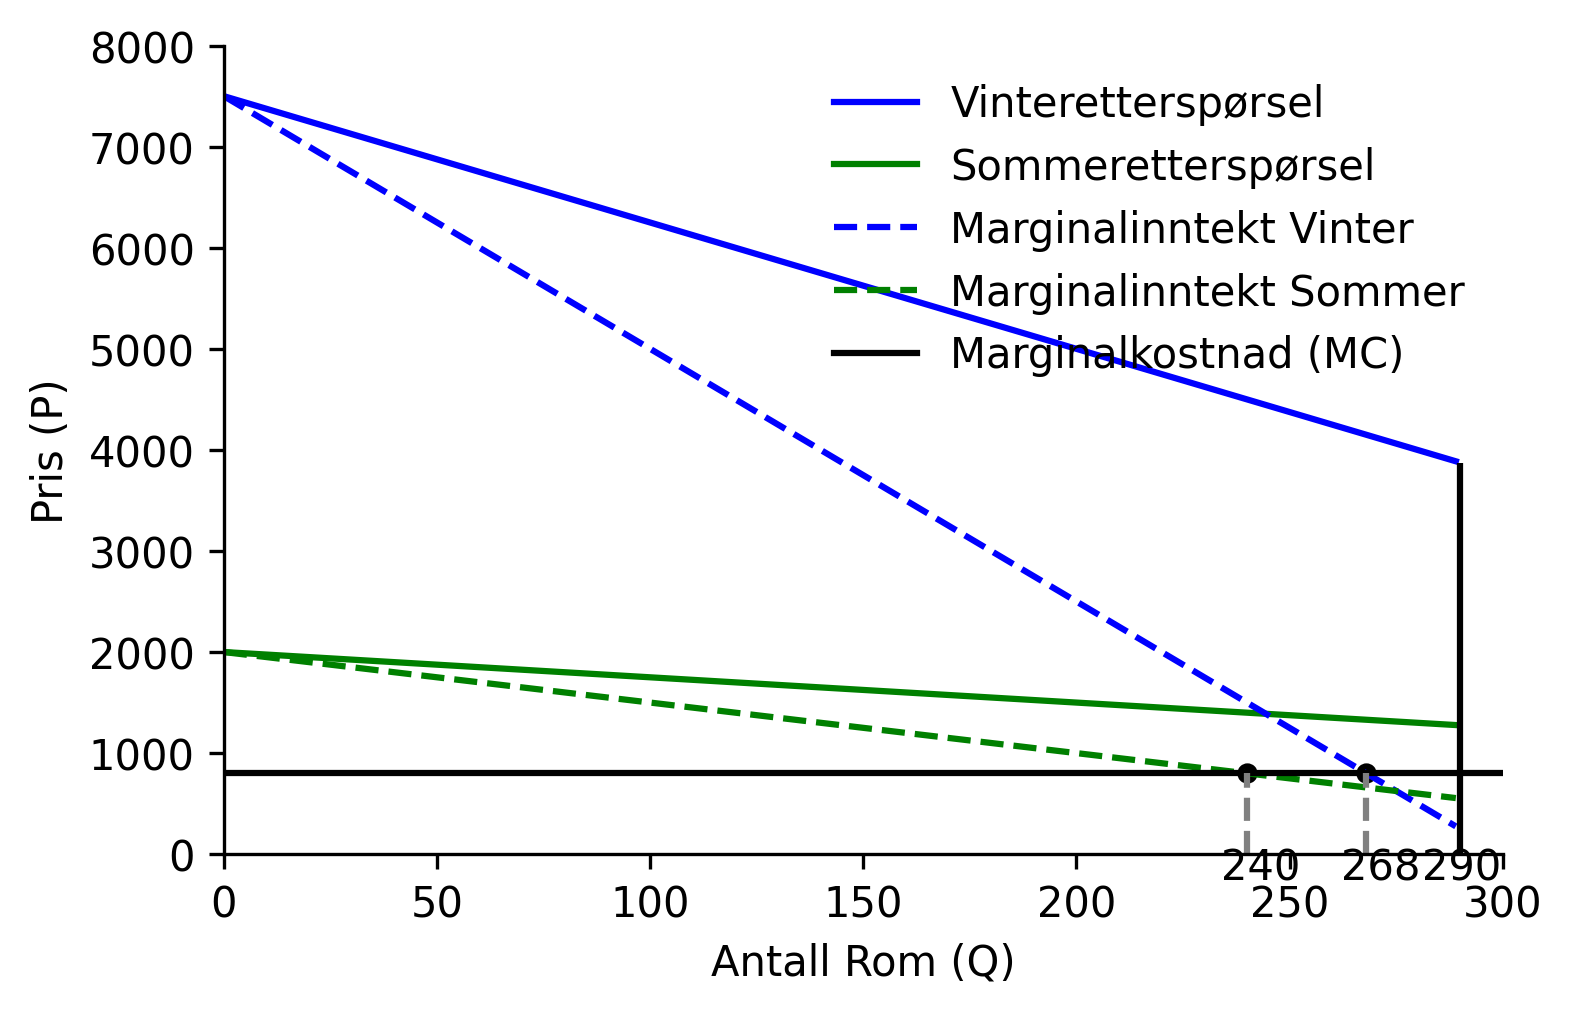
\includegraphics[width=0.48\textwidth]{dokumentobjekter/figurer/prisdiskriminering_kap3_1.png}
  \caption{Etterspørsel sommer og vinter}
  \label{fig:prisdiskriminering_kap3_1}
  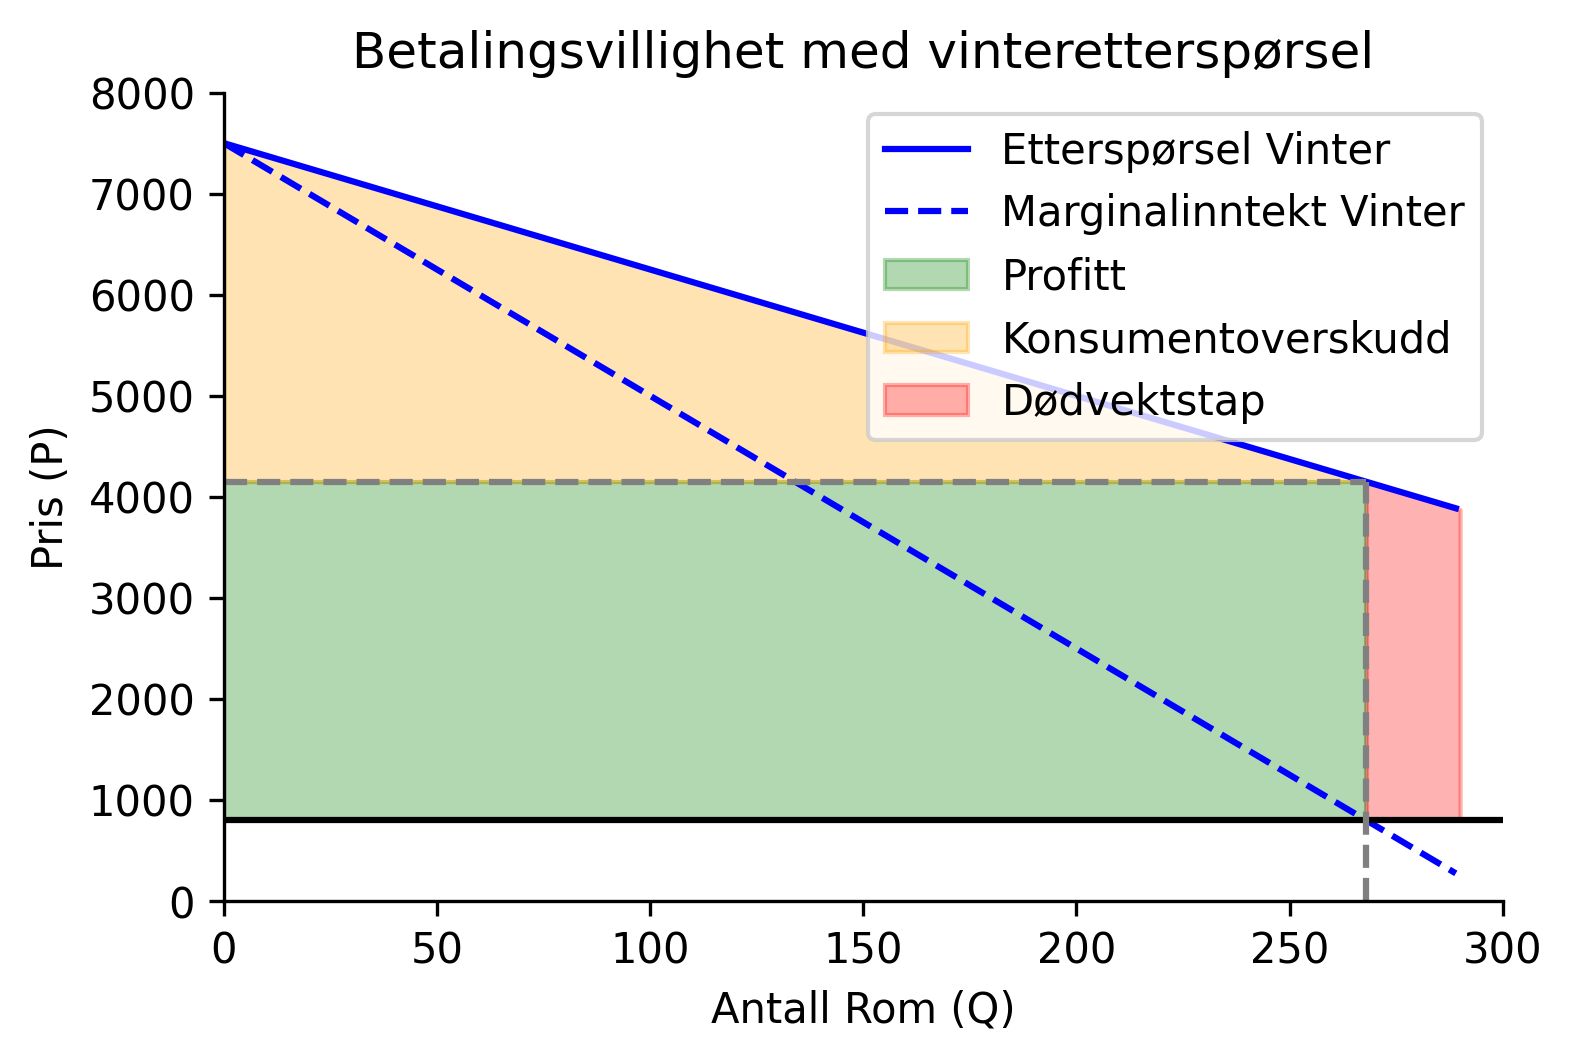
\includegraphics[width=0.48\textwidth]{dokumentobjekter/figurer/prisdiskriminering_kap3_2.png}
  \caption{Betalingsvillighet med vinteretterspørsel}
  \label{fig:vinter_ep}
  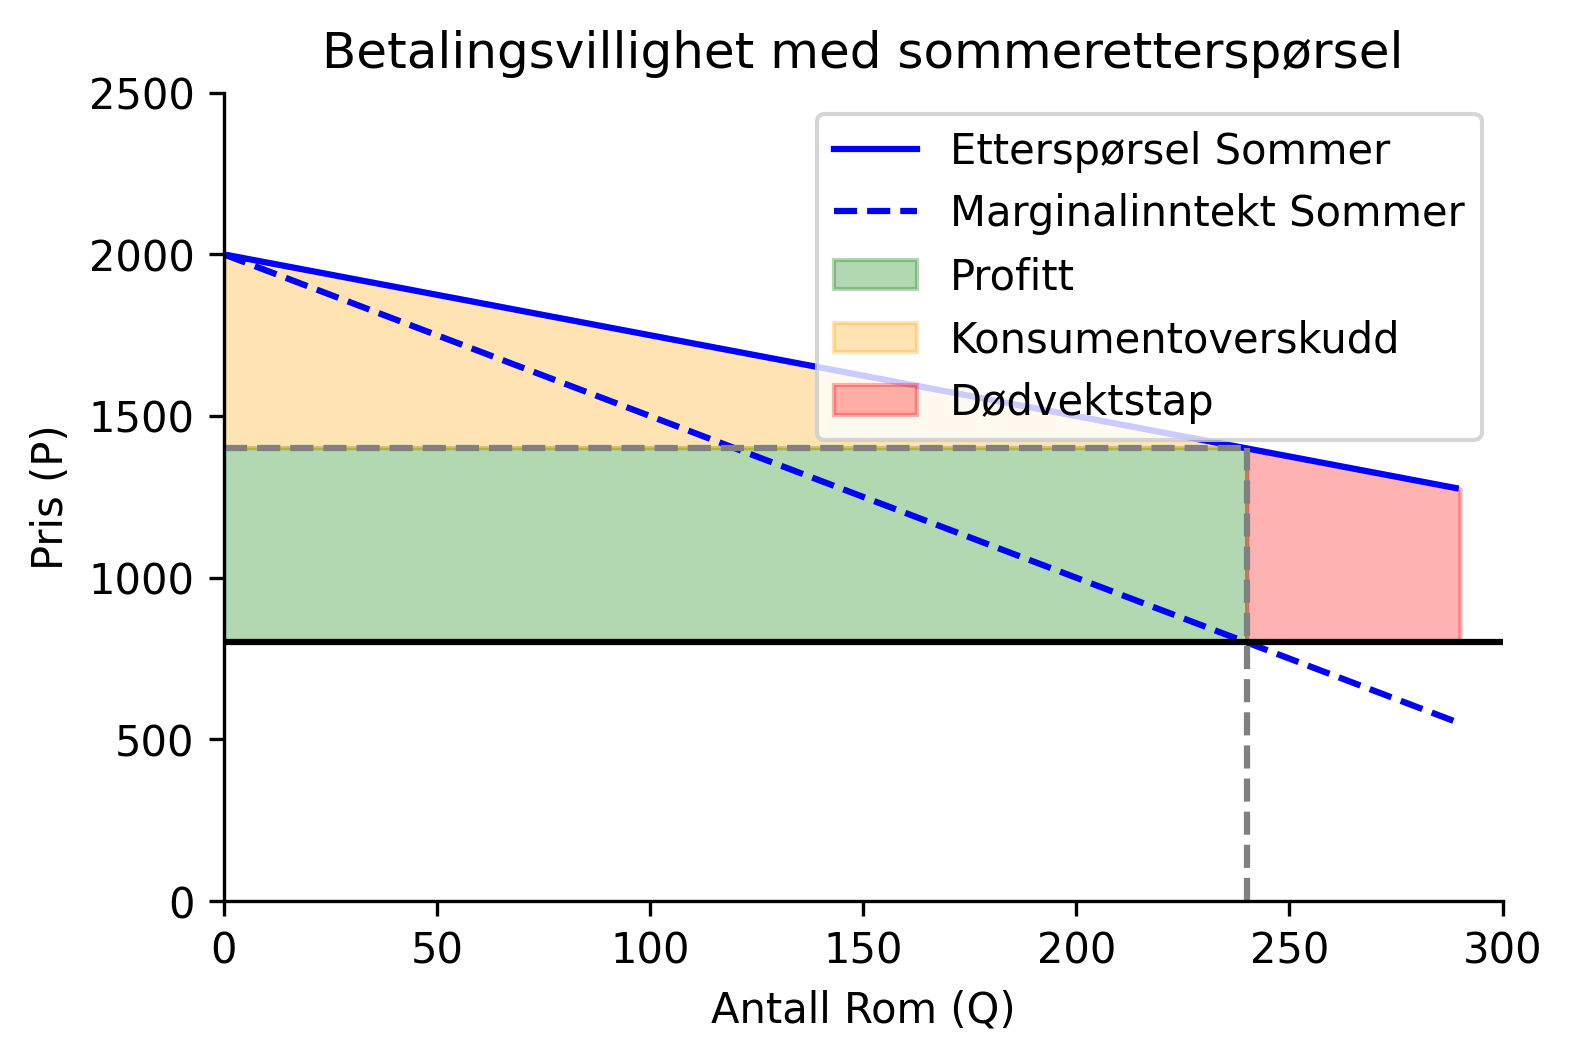
\includegraphics[width=0.48\textwidth]{dokumentobjekter/figurer/prisdiskriminering_kap3_3.png}
  \caption{Betalingsvillighet med sommeretterspørsel}
  \label{fig:sommer_ep}
  \vspace{-12mm}
\end{wrapfigure}

I \autoref{fig:prisdiskriminering_kap3_1} har vi etterspørsel for sommer
og vinter i samme figur, her kan vi se at marginalinntekten (MR) for
vinteretterspørselen er høyere enn sommeretterspørselen. Det betyr at
hotellet kan kreve en høyere pris per rom i vintermånedene.
Marginalkostnaden er satt konstant året rundt som betyr at kostnadene
for å leie ut et rom ikke endres mellom sesongene. På x--aksen kan vi se
at det optimale antallet utleide rom er 268 om vinteren og 240 om
sommeren.

\autoref{fig:vinter_ep} viser produsentoverskudd, konsumentoverskudd og
dødvekts-tap ved bruk av tredjegrads prisdiskriminering i
vintersesongen. Det grønne området er produsentoverskuddet om som er
betydelig mye større enn sommerens produsentoverskudd i
\autoref{fig:sommer_ep}. Dette skyldes høyere priser og etterspørsel om
vinteren.

Ved bruk av tredjegrads prisdiskriminering har hotellet da mulighet til
å maksimere sitt dekningsbidrag fra hotellrommene ved å tilpasse seg
optimalt til etterspørselen i de 2 sesongene.

\clearpage

I \autoref{fig:aggregert_fig} ser vi at The Edge ikke vil bruke uniform
prising siden de har en kapasitet på 290 rom. Og totalt dekningsbidrag
hypotetisk sett om de solgte alle rommene ville vært vært siden under
uniform prising blir dekningsbidraget:
\(508Q \cdot (1858P-800MC) = 537721\).

\begin{figure}[h]
  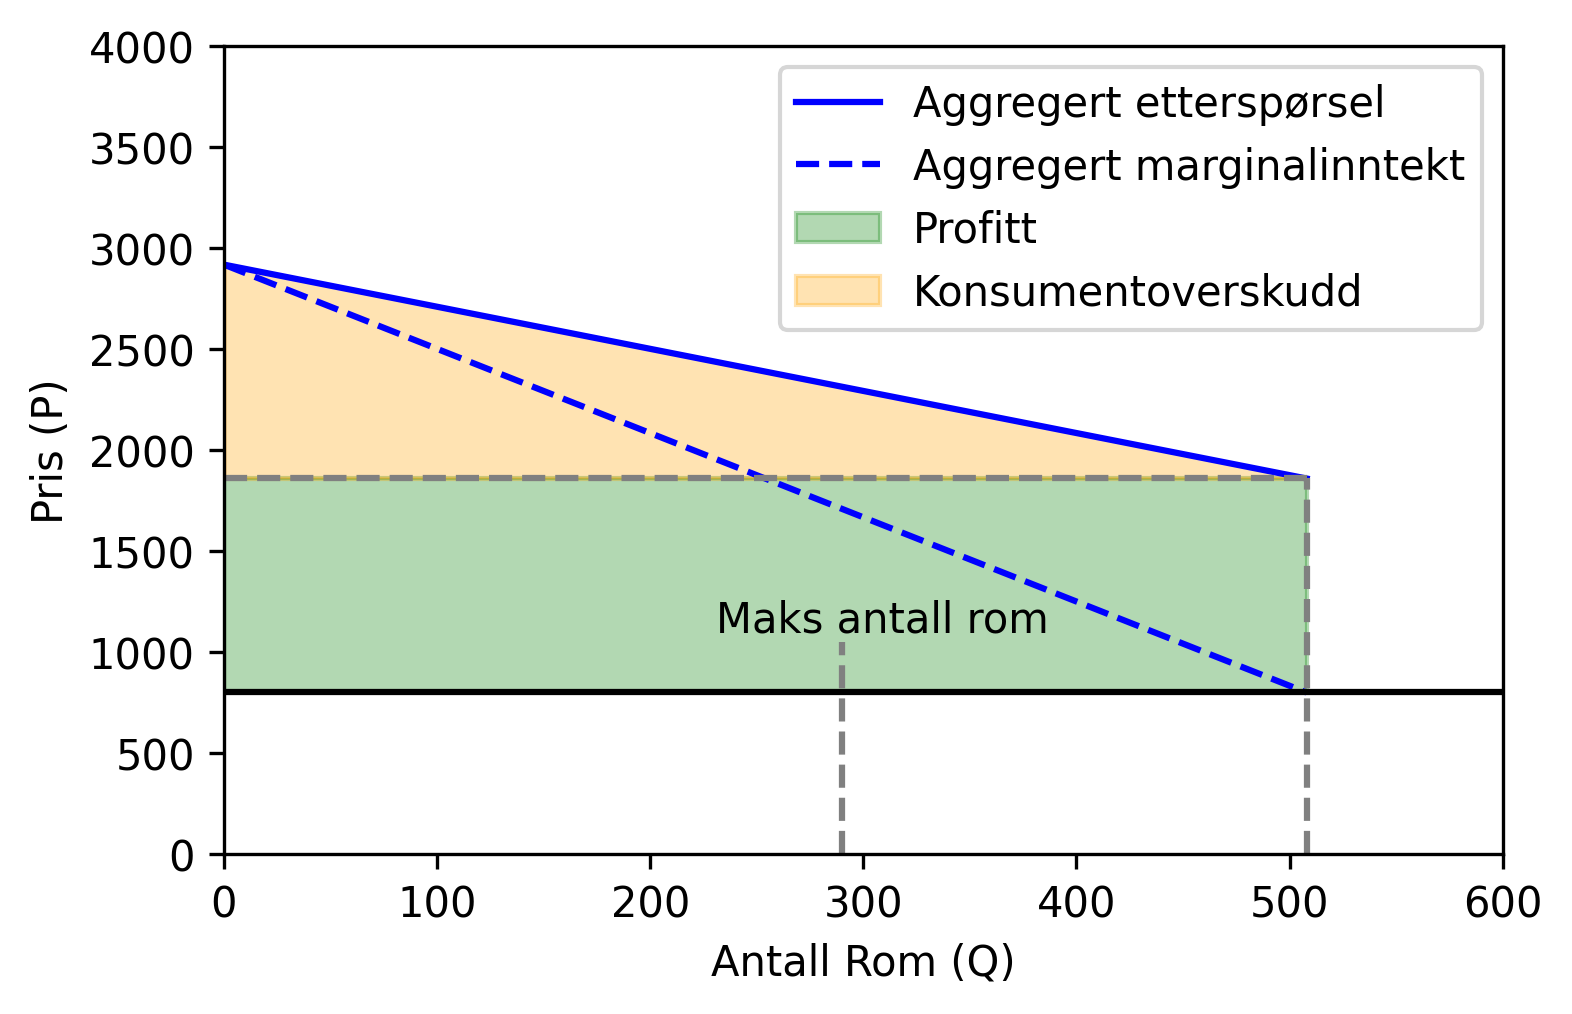
\includegraphics[width=0.9\textwidth]{dokumentobjekter/figurer/aggregert_fig.png}
  \caption{Aggregert etterspørsel}
  \label{fig:aggregert_fig}
\end{figure}

\begin{table}[h]
\centering
\begin{tabular}{|c|p{3cm}|c|p{3cm}|c|}
\hline
Sesong & Optimalt antall rom (Q) & Optimal pris (P) & Dekningsbidrag per solgte rom & Total dekningsbidrag \\
\hline
Vinter & 268 & 4150 & 3350 & 897800\\
\hline
sommer & 240 & 1400 & 600 & 144000 \\
\hline
Total & - & - & - & 1041800 \\
\hline
\end{tabular}
\caption{Med prisdiskriminering}
\label{table:med_diskrim}
\end{table}

I \autoref{table:med_diskrim} ser vi at med prisdiskrimineringen så får
vi solgt 268 rom på vinteren til en pris på 4150 og sommeren 240 rom til
en pris på 1400, totalt får hotellet inn 1.041.800 kroner i
dekningsbidrag.

\begin{table}[h]
\centering
\begin{tabular}{|c|p{3cm}|c|p{3cm}|c|}
\hline
Sesong & Optimalt antall rom (Q) & Optimal pris (P) & Dekningsbidrag per solgte rom & Total dekningsbidrag \\
\hline
Vinter & 290 & 2312.6 & 1516.6 & 439814\\
\hline
Sommer & 0 & 2312.6 & 0 & 0 \\
\hline
Total & - & - & - & 439814 \\
\hline
\end{tabular}
\caption{Uten prisdiskriminering}
\label{table:uten_diskrim}
\end{table}

Mens i \autoref{table:uten_diskrim} uten prisdiskriminering blir det
solgt 290 rom på vinteren og ingen på sommeren så da får de nå kun inn
439.814 kroner i salg av hotellrom, som er grunnen til at The Edge vil
bruke tredjegrads prisdiskriminering.

\clearpage

\subsubsection{Effekt av økt
etterspørsel}\label{effekt-av-uxf8kt-etterspuxf8rsel}

\begin{wrapfigure}{r}{0.5\textwidth}
  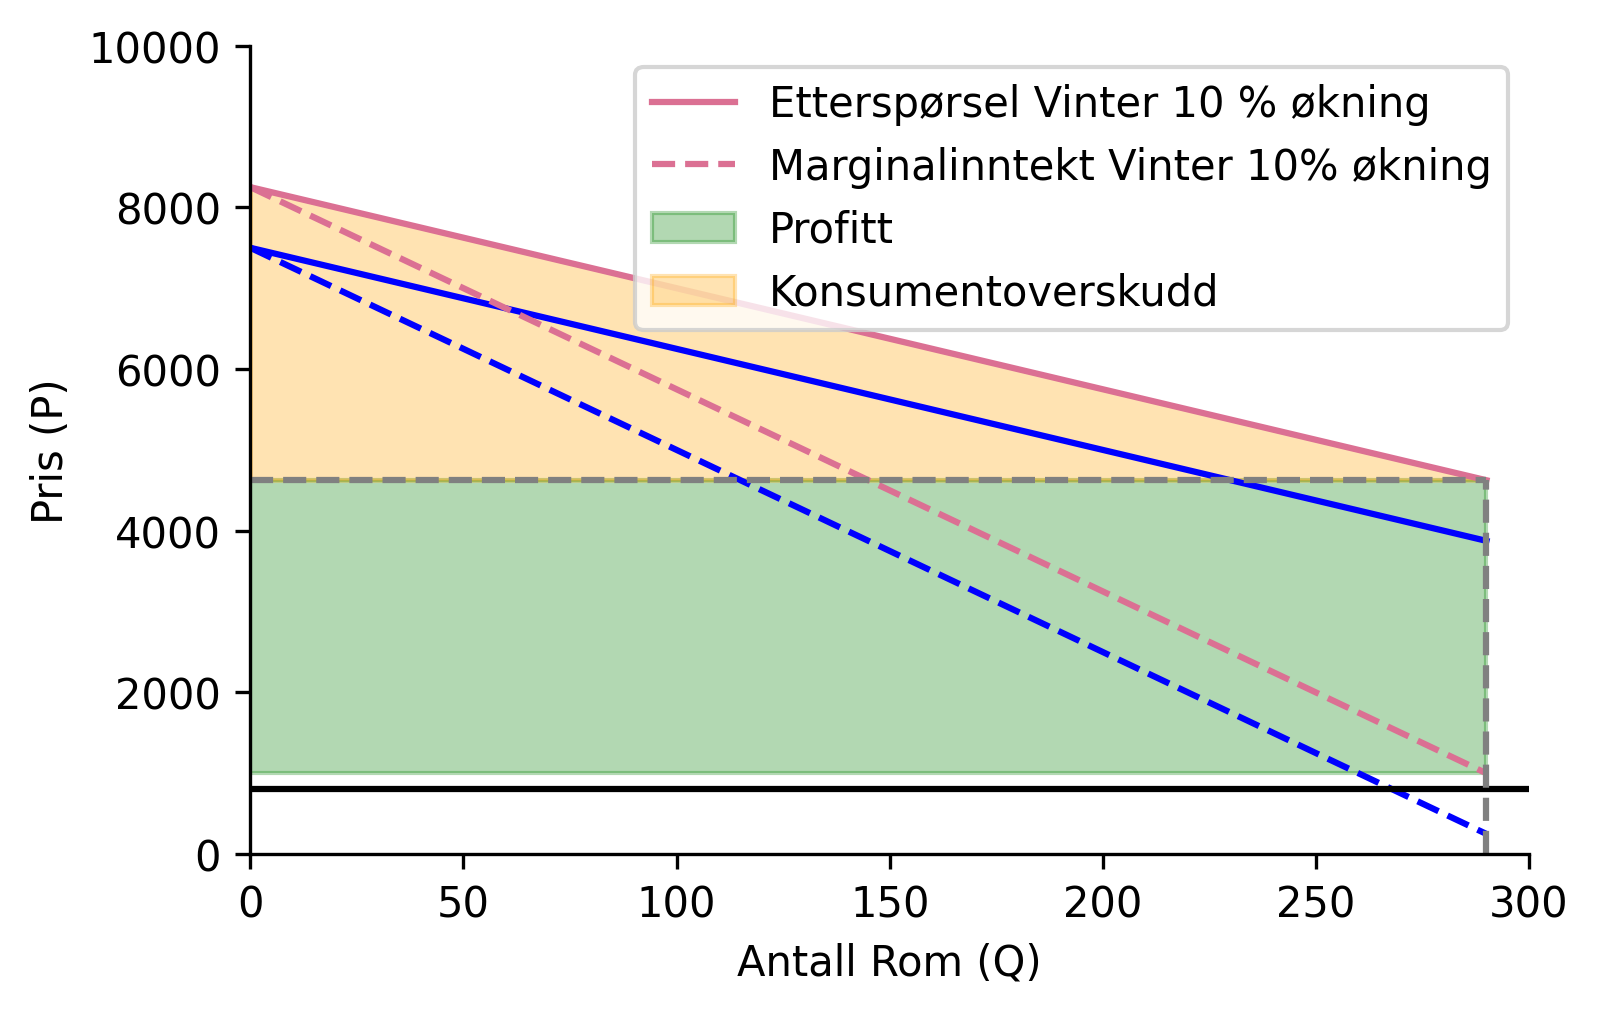
\includegraphics[width=0.48\textwidth]{dokumentobjekter/figurer/prisdiskriminering_vinter_okning_.png}
  \caption{Ti prosent økning i etterspørsel vinter}
  \label{fig:okning_ep_vinter}
  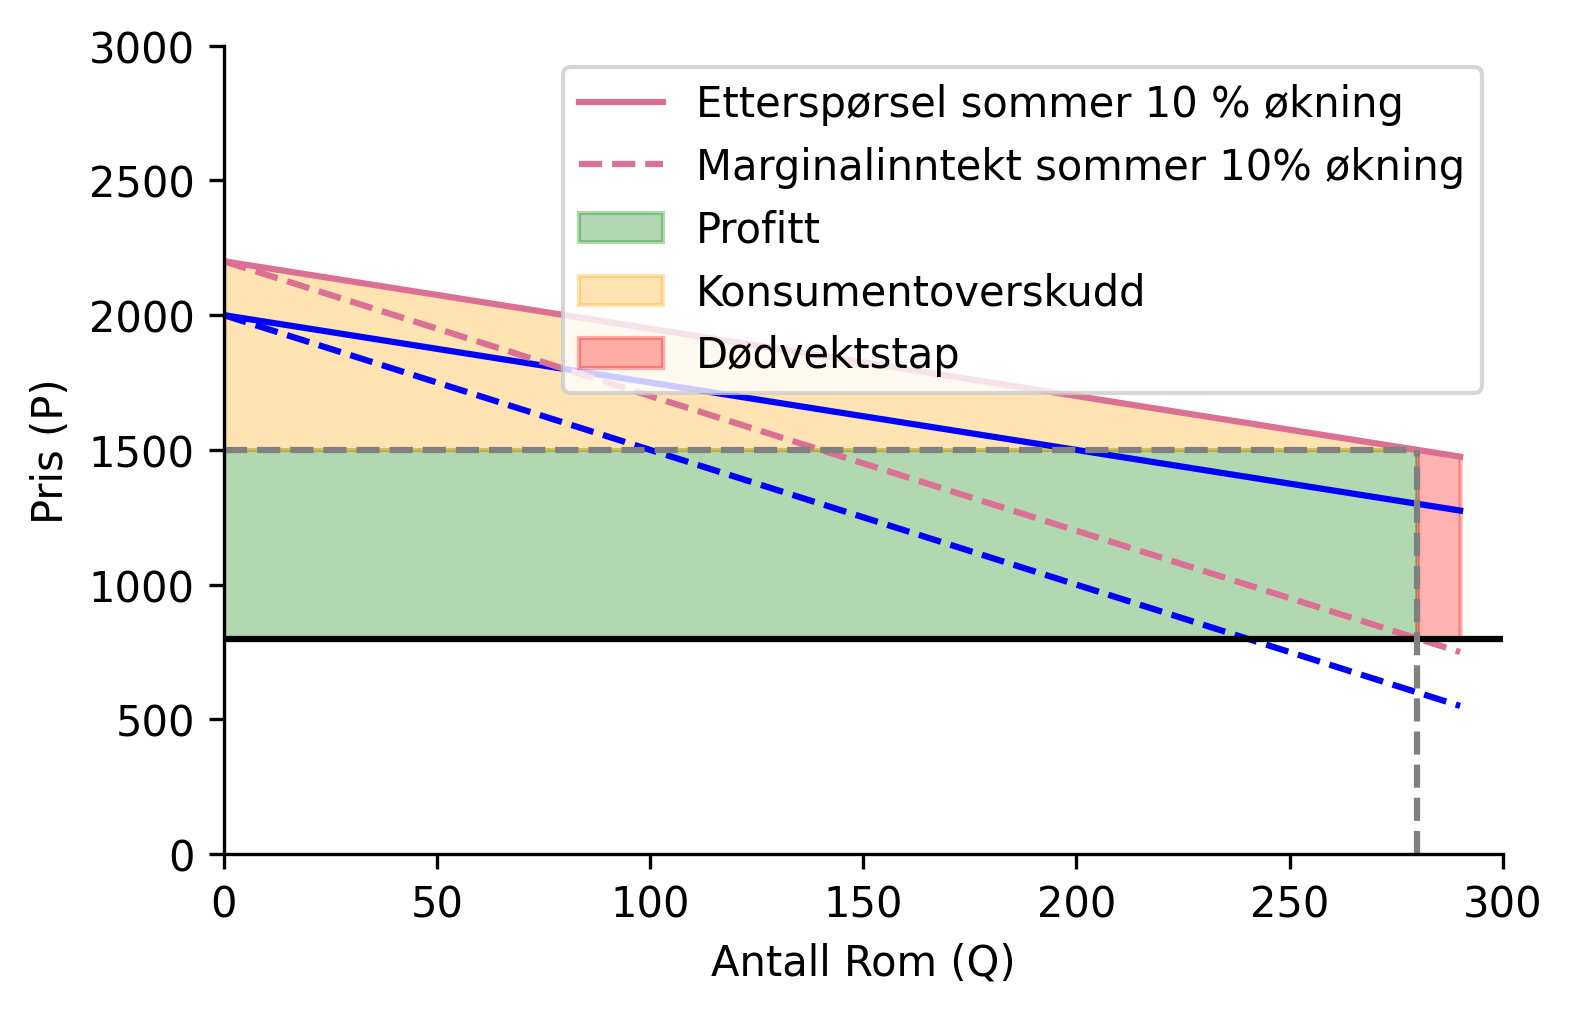
\includegraphics[width=0.48\textwidth]{dokumentobjekter/figurer/prisdiskriminering_sommer_okning_.png}
  \caption{Ti prosent økning i etterspørsel sommer}
  \label{fig:okning_ep_sommer}
  \vspace{-12mm}
\end{wrapfigure}

Analysere hvordan en økning i etterspørselen av hotellrom vil endre på
markedstilpasningen for hotellet.

\(MR = A-2BQ\), hvor \(A\) er konstantleddet og her ganges nå det inn en
økning i etterspørsel på ti prosent. Dette gir oss nå følgende
funksjoner for etterspørsel og marginalinntekt til vintersesongen:

\(P_v = (7500 \cdot 1.1) - 12.5Q_v\)

\(MR_v = (7500 \cdot 1.1) - 25Q_v\)

Og følgende til sommersesongen:

\(P_s = (2000 \cdot 1.1) - 2.5Q_s\)

\(MR_s = (2000 \cdot 1.1) - 5Q_s\)

Optimalt kvantum for vinter vil være følgende:

\(MR_v = MC \rightarrow 8250 - 25Q_v = 800 \rightarrow 25Q_v = 8250 - 800 \rightarrow Q_v = 298\)

Dette sier oss at optimalt kvantum for vintersesongen for The Edge er
298 rom solgt, men siden kapasiteten til The Edge er 290 rom så setter
vi dette som maks antall rom solgt. La oss videre regne optimalt kvantum
for sommersesongen:

\(MR_s = MC \rightarrow 2200 - 5Q_s = 800 \rightarrow 2200 - 800 = 5Q_s \rightarrow Q_s = 280\)

Som vil si at optimalt kvantum for sommersesongen blir nå 280 rom solgt
med endringen i etterspørsel på sommeren. Videre kan vi sette inn
optimalt kvantum under monopoltilpasning i de opprinnelige
etterspørselen for å finne optimal pris for The Edge:

\[P_v = 8250 - 12.5Q_v \rightarrow P_v = 8250 - 12.5 * 290 \rightarrow P_v = 8250 - 3625 \rightarrow P_v = 4625\]

\[P_s = 2200 - 2.5Q_s \rightarrow P_S = 2200 - 2.5 * 280 \rightarrow P_s = 2200 - 700 \rightarrow P_s = 1500\]

Optimal pris under vintersesongen vil være \(4625,-\) NOK pr. rom og
optimalt kvantum under samme sesong vil være 290 rom. Under
sommersesongen vil optimal pris være \(1500,-\) NOK pr. rom og optimalt
kvantum 280 rom.

\autoref{fig:okning_ep_vinter} ser vi at dødvektstapet forsvinner siden
optimalt kvantum blir satt til 290. I \autoref{fig:okning_ep_sommer} får
vi et litt mindre dødvektstap og kvantum solgt nærmer seg
maksimalkapasitet på hotellet der også. Totalt sett så ser vi at på
sommeren parallelskyves etterspørsel og maringalinntektskurvene med 200
kroner. Og for vinteren så parallelforskyves det også, men siden
etterspørselen er høyere så er det en større økning for kurvene på 750
kroner.

\clearpage

\subsubsection{Endring i elastisiteten}\label{endring-i-elastisiteten}

\begin{wrapfigure}{r}{0.5\textwidth}
  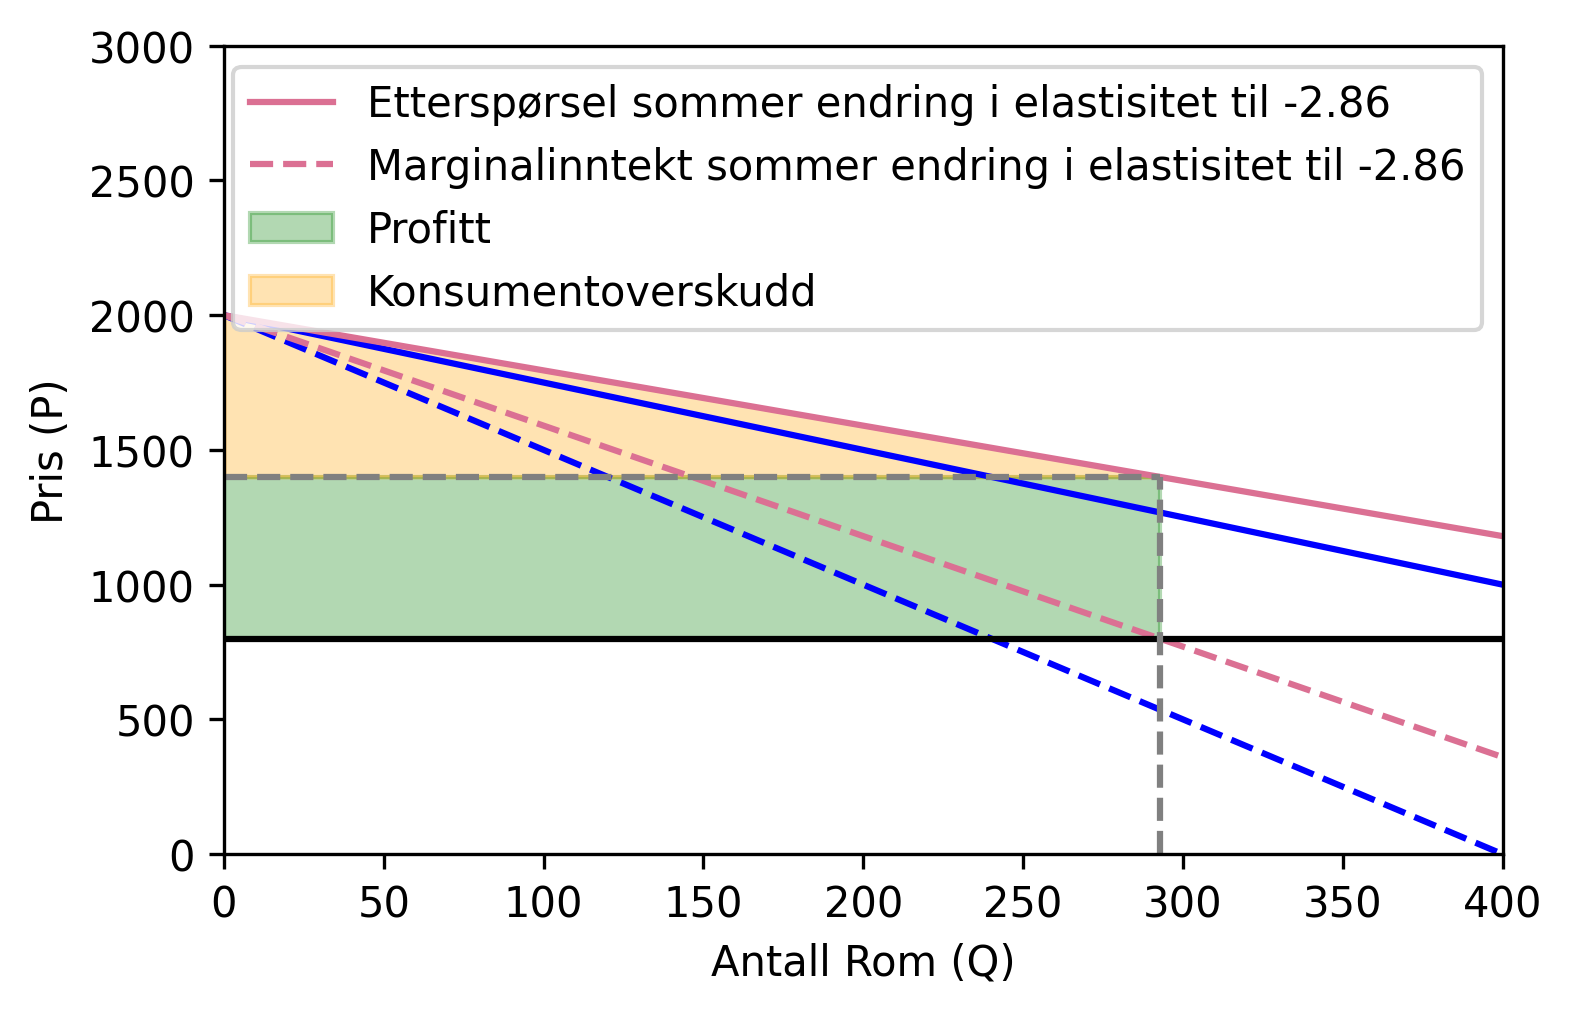
\includegraphics[width=0.48\textwidth]{dokumentobjekter/figurer/prisdiskriminerin_elas_sommer.png}
  \caption{Endring i elastisitet på lang sikt sommer}
  \label{fig:elas_sommer_kort}
  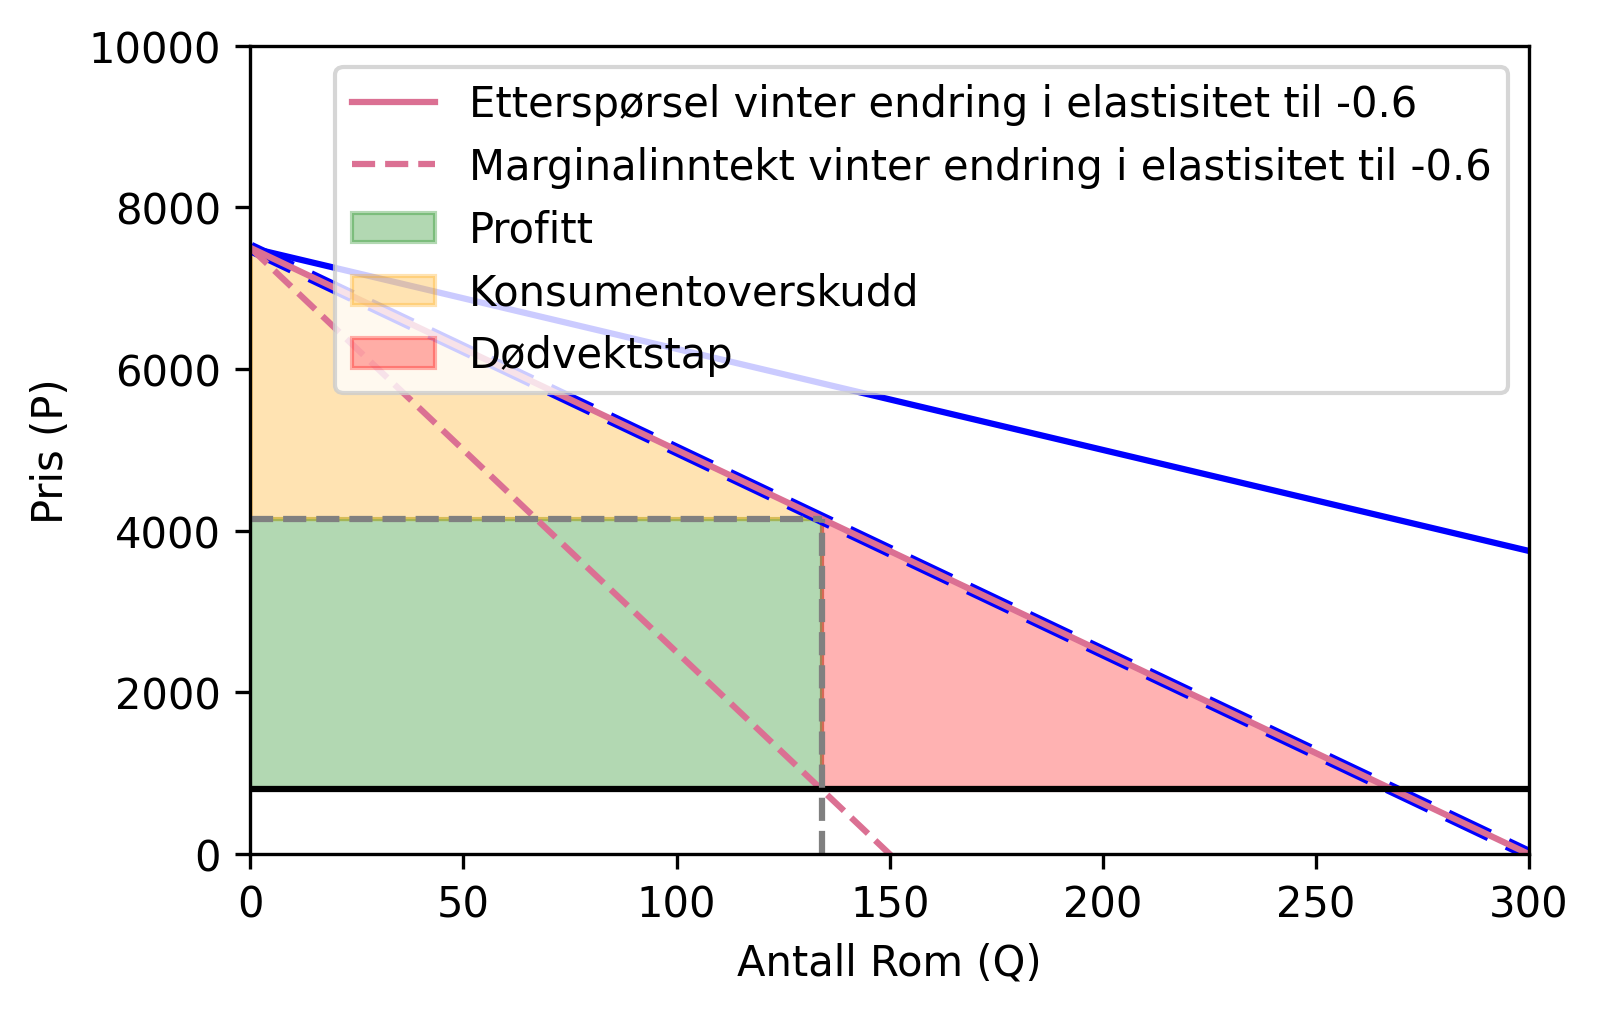
\includegraphics[width=0.48\textwidth]{dokumentobjekter/figurer/prisdiskriminering_elas_vinter}
  \caption{Endring i elastisitet på kort sikt vinter}
  \label{fig:elas_vinter_lang}
  \vspace{-14mm}
\end{wrapfigure}

I de originale etterspørselsfunksjonene for sommer og vintersesong så
finner vi elastisitetene ved å først løse sette ligningene som en
funksjon av pris og løse for kvantum:

\(P_V = 7500 - 12.5 \cdot Q \rightarrow E_V = 600 - 0.08P\)

\(P_S = 2000 - 2.5 \cdot Q \rightarrow E_S = 800 - 0.4P\)

Deretter finner vi den deriverte av etterspørselsfunksjonene:

\(E_V = 600 - 0.08P \rightarrow \frac{dE_V}{dP} = -0.08\)

\(E_S = 800 - 0.4P \rightarrow \frac{dE_S}{dP} = -0.4\)

og for å finne priselastisiteten så ganger vi med inntekt og deler på
kvantum:

\(E_V = -0.08 \cdot \frac{4150}{268} = -1.24\)

\(E_S = -0.4 \cdot \frac{1400}{240} = -2.33\)

og finner da at på sommersesongen så er elastisiteten -2.33, mens på
vinteren er elastisiteten -1.24, som betyr at etterspørselen her er
elastisk for begge årstidene.

Tidligere nevnt i
\href{https://ntnuopen.ntnu.no/ntnu-xmlui/bitstream/handle/11250/2486498/Masteroppgave\%20Ida\%20Charlotte\%20Engebretsen.pdf}{Ida Charlotte Sølvberg Engebretsen}
sin masteroppgave har hun estimert prisfølsomhet til turister på -0.6 på
kort sikt og -2.86 på lang sikt.

Ved på endre på parameteren B i etterspørsellikningene for sommer og
vinter:

\(P_V = 7500 - 25 \cdot Q \rightarrow E_V = 298 - 0.04P\)

\(P_S = 2000 -2.84 \cdot Q \rightarrow E_S = 975 - 0.487P\)

kan vi se på elastisiteter som er ganske like de Ida estimerte i sin
masteroppgave (her gjøres det en antakelse at pris og kvantum er det
samme):

\(E_V = -0.04 \cdot \frac{4150}{268} = -0.616\) og lang sikt for
sommeren: \(E_S = -0.487 \cdot \frac{1400}{240} = -2.84\)

kan vi se at på sommeren med en større økning i prisfølsomhet vil The
Edge gå fra å selge 240 rom opprinnelig til å nå faktisk dekke alle 290
rommene sine med samme pris på 1400.

På vinteren endres elastisiteten fra -1.24 til ca -0.61 og
etterspørselen går fra elastisk til uelastisk og etterspørselskurven
blir mye brattere, The Edge har nå en nedgang på vinteren fra 268 rom
solgt til 134.

\clearpage

\subsection{3.3 Diskusjon}\label{diskusjon}

\subsubsection{Hvilken effekt kan vi se}\label{hvilken-effekt-kan-vi-se}

I \autoref{fig:konsum} så ser vi at det har vært en økning i
turistkonsum i Norge, hvor det spesielt har vært en økning i periodene
der kronen har blitt svakere. Dette kan være en indikasjon på at
turister er prisfølsomme. Men som beskrevet i
\hyperlink{faktorer_ettersporsel}{kapittel 1.3 faktorer som påvirker etterspørsel}
så ser vi en etterspørselselastisitet på -0.6 på kort sikt og -2.86 på
lang sikt. Så når det nå har blitt billigere for turister å reise til
Norge muligens begrunnet en svak kronekurs, har turistkonsumet her til
lands økt. Dette kan potensielt forklare noe av den øke etterspørselen
man kan observere, spesielt i Tromsø. Begrenset kapasitet, og høy
etterspørsel driver prisene høyt.

\subsubsection{Optimal prisstrategi}\label{optimal-prisstrategi}

Som vi kunne observere i \autoref{table:uten_diskrim}, ville en uniform
pris på 2312,6 kroner per natt medføre at The Edge ikke fikk solgt noen
rom under sommersesong, gitt etterspørselen. På vinteren ville alle 290
rommene blitt solgt.

Om The Edge velger å benytte seg av tredjegradsprisdiskriminering ville
hotellet kunne selge rom både om vinteren og sommeren til ulike priser,
som illustrert i \autoref{table:med_diskrim}. Hotellet vil dermed få et
økt dekningsbidrag om vinteren, da prisen vil øke fra 2312,6 kr per rom
til 4150 kr per rom. Om sommeren vil The Edge kunne tilpasse seg den
lavere etterspørsel, og fortsatt selge rom med overskudd. Prisen om
sommeren vil være lavere enn vintersesongen, grunnet den lavere
etterspørselen. Her vil optimal pris være 1400 kr per rom, i stedet for
den uniforme prisen på 2312,6kr per rom. Da vil The Edge fortsatt få
salg om sommeren, og på et positivt dekningsbidrag under denne sesongen
også.

Den optimale prisstrategien for The Edge vil dermed være tredjegrads
prisdiskriminering istedet for uniform prising. Med en inntekt på 4150
NOK og 1400 NOK per rom avhengig av sesongen, og konstant enhetskostnad
på 800 kr per rom. Dersom The Edge skulle tatt en uniform pris for hele
året, ville hotellet gått glipp av potensielle lønnsomme salg om
sommeren, samt miste mye potensielt overskudd som de klarer å hente om
vinteren ved å benytte en høyere pris under denne sesongen, gitt at
etterspørselen forholder seg høy.

\subsubsection{Monopol-antakelsen}\label{monopol-antakelsen}

I vår analyse antok vi at The Edge var en monopolist innenfor sitt
segment (High-end luxury, konferanse). Innenfor segmentet kan det finnes
hoteller med potensielt substituerbare goder, blant annet Radisson Blue
og Scandic Ishavshotel. Selv om hotellene ikke har samme karakteristiske
utseende, eller samme merkevare, kan det virke som disse blant annet
konkurrerer innenfor konferansehotellmarkedet. Derfor må denne
antakelsen taes hensyn til i analysen vår. Dersom man antok konkurranse,
ville ikke The Edge stå ovenfor hele etterspørselen, og dermed ikke
kunne sette prisen selv grunnet at prisene til eventuelle konkurrenter
vil påvirke.

\subsubsection{Dynamisk prising gjennom
Mews}\label{dynamisk-prising-gjennom-mews}

The Edge benytter seg også av Mews sine systemer, som antatt
innledningskapitlet. Kombinert med at the Edge setter høyere basepris
under vintersesongen, vil også prisene justeres utifra hvor mange rom
som er solgt. Dette vil si om The Edge har solgt halvparten av rommene,
vil prisen være høyere enn om bare en tiendedel var solgt (gitt av dette
var samme dag/sesong). At Mews automatisk oppjusterer priser kan påvirke
solgt kvantum dersom de som etterspør hotellrom er prissensetiv, noe
trenden med svekket kronekurs/økt konsum av utenlandske i Norge kan
implikere. Dersom dette er case, kunne eventuelt denne automatiske
oppjusteringen ha en negativ effekt på solgt kvantum. Samtidig dersom
konsumentene ikke er sensitiv til pris, vil derimot denne automatiske
økte prisen kunne øke dekningsbidraget.

\subsubsection{Virkeligheten}\label{virkeligheten}

Som vi kunne se i analysedelen, vil The Edge få økt sitt dekningsbidrag
ved å benytte tredjegrads prisdiskriminering. Men hvordan samsvarer
dette med det vi kan observere i data med hotellrompriser i Tromsø? I
\autoref{fig:ssbdata} så vi at prisene varierte basert på sesong. Selv
om dette ikke er spesifikt til Clarion Hotel The Edge, kan de se ut som
bransjen som helhet har valgt å ta en høyere pris under vintersesong.
Dette kan igjen indikere at bransjen har begynt å anvende tredjegrads
prisdikskriminering til noen grad, spesielt i forhold til tidligere. Vi
kan alikevell ikke si at dette er den eneste grunnen til den økte
prisen, gitt at vi er i en periode med relativ høy inflasjon.

Et argument som kan være med å støtte at bransjen som helhet har startet
å anvende prisdiskriminering er driftsmarginene. Som nevnt i
innledningen, kunne NHO presentere økte driftsmarginer for bransjen. I
2019 var denne på 1,9 prosent, og har siden økt til 3,9 prosent, en
relativ økning på over 100 prosent. Selv om prisdiskriminering alene er
årsak, kan dette være en av faktorene.\footnote{\emph{Tall Og Fakta Om
  Norsk Reiseliv} (n.d.)}

\subsubsection{Til slutt}\label{til-slutt}

Teorien for aggregert etterspørsel lar seg ikke gjøre med The Edge,
grunnet kapasitetsbegrensninger. Disse kapasitetsbegrensningene fører
til at sommersesongen ikke gir hotellet dekningsbidrag grunnet at prisen
er høyere (dersom The Edge skal ha uniform pris) enn konsumentene har
betalingsvillighet for. Derfor vil tredjegradspridiskriminering gi The
Edge en løsning, hvor hotellet tilpasser seg prismessig basert på
etterspørselen fra de ulike sesongene. Ut ifra tallene fra
driftsmarginer fra NHO, at driftsmarginen nesten har doblet seg (1,9
prosent til 3,9 prosent) og den økte prisen under vintersesong, kan vi
anta at hotellene har valgt å ta ulik pris basert utifra etterspørselen.
Om vinteren er etterspørselen høyere, og dermed hotellene har økt sine
hotellrompriser under vintersesong, som vil si at det kan se ut som
hotellene har valgt å prisdiskriminere basert på sesong.

\clearpage

\section{4. Konklusjon}\label{konklusjon}

\subsection{Hovedfunn}\label{hovedfunn}

Denne oppgaven har undersøkt hvilken effekt prisdiskriminering ville
hatt på lønnsomheten og markedstilpasningen til Clarion Hotel The Edge
med fokus på sesongbaserte variasjoner på etterspørsel. Med dataanalyse
i kapittel 1 og teori i kapittel 2 har vi i kapittel 3 demonstrert
hvordan tredjegradsprisdiskriminering kan forbedre hotellets økonomiske
resultat og redusere dødvektstap gitt kapasitetsbegrensningen, noe som
øker det samfunnsøkonomiske overskuddet.

Dersom The edge hadde valgt en form for uniform prising basert på
aggregert etterspørsel så ville de ikke solgt noen rom på sommeren men
solgt ut alle rommene på vinter til lavere pris enn det ville kommet i
en markedslikevekt. Men dersom de hadde valgt en annen prisstrategi
basert på sesongmessig etterspørsel gjør det at hotellet selger rom til
en høyere pris på vinter og selger ut nesten hele sin kapasitet på
sommer til en lavere pris. Ved å benytte en slik strategi så maksimerer
hotellet sin kapasitetsutnyttelse og inntjening i vintersesong samtidig
som det sikrer et tilfredsstillende hotellbelegg i sommersesongen.

\subsubsection{Økt etterspørsel}\label{uxf8kt-etterspuxf8rsel}

Vi ser også at mye tyder på at det vil komme økt etterspørsel delvis pga
for eksempel flere hetebølger i Europa, og en svakere kronekurs. Men vi
har også sett at etterspørselselastisiteten er elastisk på lang sikt så
dersom hotellene setter prisene for høyt, så kan det hende at turismen
reduseres på lang sikt slik at de blir nødt til å sette ned pris for å
oppnå samme kvantum.

\subsection{4.2 Videre analyse}\label{videre-analyse}

\subsubsection{Flere hoteller}\label{flere-hoteller}

Siden vi i denne oppgaven ikke har sett på tilbudssiden så vil videre
analyse være nødvendig for å få utforsket hvordan den høye marginen
mellom kostnad og pris kan føre til nye aktører på markedet, som ville
økt hotellrom kapasiteten og ført til en ny markedslikevekt med lavere
priser.

\subsubsection{Dynamisk prising}\label{dynamisk-prising}

Som vi så med MEWS så kan det også være nødvendig med undersøkelse av
mer avansert prisstrategier som dynamisk prising basert på sanntidsdata.

\subsubsection{Betalingsvillighet}\label{betalingsvillighet}

Det har vært snakk om at utenlandske turister har enn høyere
betalingsvillighet, og oppgaven vi brukte for etterspørselselasisiteten
begynner nå å bli utdatert så det kan være nødvendig med ny analyse på
elasisiteten og betalingsvilje for utenlandske turister i forhold til
norske.

\clearpage

\section{Referanser}\label{referanser}

\phantomsection\label{refs}
\begin{CSLReferences}{1}{0}
\bibitem[\citeproctext]{ref-engebretsen_2017_norge}
Engebretsen, I. C. S. (2017). \emph{Norge som reisemål: Effekten av
inntekt, pris og valutakurs på utenlandsk etterspørsel - en empirisk
studie for perioden 1995-2015}. ntnuopen.ntnu.no.
\url{https://ntnuopen.ntnu.no/ntnu-xmlui/handle/11250/2486498}

\bibitem[\citeproctext]{ref-finansdepartementet_2019_nou}
Finansdepartementet. (2019). \emph{NOU 2019: 11}. Regjeringen.no.
\url{https://www.regjeringen.no/no/dokumenter/nou-2019-11/id2645213/?ch=7}

\bibitem[\citeproctext]{ref-kandidatnummer_2023_mappeoppgave}
Kandidatnummer\_3. (2023). \emph{Mappeoppgave 1 -samfunnsøkonomisk
analyse av en turistskatt} (pp. 8--10).

\bibitem[\citeproctext]{ref-mews_hotel}
Mews. (n.d.-a). \emph{Hotel rate management software \textbar{} mews}.
www.mews.com. Retrieved March 18, 2024, from
\url{https://www.mews.com/en/products/hotel-rate-management}

\bibitem[\citeproctext]{ref-mews_strawberry}
Mews. (n.d.-b). \emph{Strawberry customer story \textbar{} mews case
study}. www.mews.com. Retrieved March 18, 2024, from
\url{https://www.mews.com/en/customers/strawberryhotels}

\bibitem[\citeproctext]{ref-michalsen_2024_naeringskonomi3}
Michalsen, A. (2024a). \emph{• lineaer prising og tredje grads
prisdiskriminering • velferdseffekter}.
\url{https://uit-sok-2030-v24.github.io/Forelesning\%203\%20-\%20monopol\%20og\%20prisdiskriminering.pdf}

\bibitem[\citeproctext]{ref-michalsen_2024_naeringskonomi2}
Michalsen, A. (2024b). \emph{Naeringsøkonomi og konkurransestrategi}.
\url{https://uit-sok-2030-v24.github.io/Forelesning\%202\%20-\%20grunnleggende\%20mikr\%C3\%B8konomi.pdf}

\bibitem[\citeproctext]{ref-michalsen_2024_naeringskonomi4}
Michalsen, A. (2024c). \emph{Naeringsøkonomi og konkurransestrategi}.
\url{https://uit-sok-2030-v24.github.io/Forelesning\%204\%20-\%20monopol\%20og\%20prisdiskriminering.pdf}

\bibitem[\citeproctext]{ref-michalsen_2024_naeringskonomi5}
Michalsen, A. (2024d). \emph{Naeringsøkonomi og konkurransestrategi}.
\url{https://uit-sok-2030-v24.github.io/Forelesning\%205\%20-\%20monopol,\%20produktvalg\%20og\%20kvalitet.pdf}

\bibitem[\citeproctext]{ref-michalsen_2024_naeringskonomi6}
Michalsen, A. (2024e). \emph{Naeringsøkonomi og konkurransestrategi}.
\url{https://uit-sok-2030-v24.github.io/Forelesning\%206\%20-\%20Kvantumskonkurranse\%20og\%20Cournot\%20modell\%20-\%20til\%20forelesning.pdf}

\bibitem[\citeproctext]{ref-pepall_2014_industrial}
Pepall, L., Richards, D. J. \& Norman, G. (2014). \emph{Industrial
organization : Contemporary theory and empirical applications}. Wiley.

\bibitem[\citeproctext]{ref-tall}
\emph{Tall og fakta om norsk reiseliv}. (n.d.). www.nhoreiseliv.no.
\url{https://www.nhoreiseliv.no/tall-og-fakta/tall-og-fakta-om-norsk-reiseliv/}

\end{CSLReferences}

\appendix

\section {Appendix Generell KI bruk}

I løpet av koden så kan det ses mange \# kommentarer der det er skrevet
for eks ``\#fillbetween q1 and q2''. Når vi skriver kode i Visual Studio
Code så har vi en plugin som heter Github Copilot. Når vi skriver slike
kommentarer så kan den foresøke å fullføre kodelinjene mens vi skriver
de. Noen ganger klarer den det, men andre ikke. Det er vanskelig å
dokumentere hvert bruk der den er brukt siden det ``går veldig fort''
men siden vi ikke har fått på plass en slik dokumentasjon så kan all
python kode der det er brukt kommentarer antas som at det er brukt
Github Copilot. Nærmere info om dette KI verktøyet kan ses på
\url{https://github.com/features/copilot}



\end{document}
